% Chapter 1: Data, returns and indicators
% Statistics of Financial Markets -- Bachelor's programme, Bucharest University of Economic Studies
% GENERATED by latex/build_chapter1.py -- edit the generator, not this file.

\newcommand{\coursename}{Statistics of Financial Markets}
% Preambul comun SFM -- Statistica piețelor financiare / Statistics of Financial Markets (Beamer, 16:9)
% Același design ca MFM. Înainte de % Preambul comun SFM -- Statistica piețelor financiare / Statistics of Financial Markets (Beamer, 16:9)
% Același design ca MFM. Înainte de % Preambul comun SFM -- Statistica piețelor financiare / Statistics of Financial Markets (Beamer, 16:9)
% Același design ca MFM. Înainte de \input{../../latex/preamble} se definește
%   \newcommand{\coursename}{Statistics of Financial Markets}      (EN)
%   \newcommand{\coursename}{Statistica piețelor financiare}       (RO)  și  \def\sfmlang{ro}
% Fișierele .tex se află în EN/Courses, EN/Seminars, RO/Cursuri, RO/Seminarii (două niveluri sub rădăcină).
% Deck-urile sînt generate de latex/build_chapterN.py / build_seminarN.py (vezi latex/sfm_build.py).

\documentclass[9pt, aspectratio=169, t]{beamer}
\providecommand{\coursename}{Statistics of Financial Markets}

% Ensure content fits on slides
\setbeamersize{text margin left=8mm, text margin right=8mm}

%=============================================================================
% THEME AND STYLE CONFIGURATION
%=============================================================================
\usetheme{default}
% Using default theme for clean header/footer control

% Color Palette (matching Redispatch PDF)
\definecolor{MainBlue}{RGB}{26, 58, 110}
\definecolor{AccentBlue}{RGB}{26, 58, 110}
\definecolor{IDAred}{RGB}{205, 0, 0}
\definecolor{DarkGray}{RGB}{51, 51, 51}
\definecolor{MediumGray}{RGB}{128, 128, 128}
\definecolor{LightGray}{RGB}{248, 248, 248}
\definecolor{VeryLightGray}{RGB}{235, 235, 235}
\definecolor{KeynoteGray}{RGB}{218, 218, 218}
\definecolor{SectionGray}{RGB}{120, 120, 120}
\definecolor{FooterGray}{RGB}{100, 100, 100}
\definecolor{Crimson}{RGB}{220, 53, 69}
\definecolor{Forest}{RGB}{46, 125, 50}
\definecolor{Amber}{RGB}{181, 133, 63}
\definecolor{Orange}{RGB}{230, 126, 34}
\definecolor{Purple}{RGB}{142, 68, 173}

% Gradient background (exact Keynote 315° gradient: white to RGB 218,218,218)
\setbeamertemplate{background}{%
    \begin{tikzpicture}[remember picture, overlay]
        \shade[shading=axis, shading angle=315,
        top color=white, bottom color=KeynoteGray]
        (current page.south west) rectangle (current page.north east);
    \end{tikzpicture}%
}
% Fallback solid color for compatibility
\setbeamercolor{background canvas}{bg=}

\setbeamercolor{palette primary}{bg=MainBlue, fg=white}
\setbeamercolor{palette secondary}{bg=MainBlue!85, fg=white}
\setbeamercolor{palette tertiary}{bg=MainBlue!70, fg=white}
\setbeamercolor{structure}{fg=MainBlue}
\setbeamercolor{title}{fg=IDAred}
\setbeamercolor{frametitle}{fg=IDAred, bg=}
\setbeamercolor{block title}{bg=MainBlue, fg=white}
\setbeamercolor{block body}{bg=VeryLightGray, fg=DarkGray}
\setbeamercolor{block title alerted}{bg=Crimson, fg=white}
\setbeamercolor{block body alerted}{bg=Crimson!8, fg=DarkGray}
\setbeamercolor{block title example}{bg=Forest, fg=white}
\setbeamercolor{block body example}{bg=Forest!8, fg=DarkGray}
\setbeamercolor{item}{fg=MainBlue}

% Footer colors (override Madrid theme blue)
\setbeamercolor{author in head/foot}{fg=FooterGray, bg=}
\setbeamercolor{title in head/foot}{fg=FooterGray, bg=}
\setbeamercolor{date in head/foot}{fg=FooterGray, bg=}
\setbeamercolor{section in head/foot}{fg=FooterGray, bg=}
\setbeamercolor{subsection in head/foot}{fg=FooterGray, bg=}

% Bullet styles (apply everywhere including blocks)
\setbeamertemplate{itemize item}{\color{MainBlue}$\boxdot$}
\setbeamertemplate{itemize subitem}{\color{MainBlue}$\blacktriangleright$}
\setbeamertemplate{itemize subsubitem}{\color{MainBlue}\tiny$\bullet$}
\setbeamertemplate{itemize/enumerate body begin}{\normalsize}
\setbeamertemplate{itemize/enumerate subbody begin}{\normalsize}

% Item spacing - compact style
\setlength{\leftmargini}{10pt}       % Level 1: minimal indent
\setlength{\leftmarginii}{10pt}      % Level 2: minimal additional indent
% Compact list spacing (zero extra space before/after lists in blocks)
\makeatletter
\def\@listi{\leftmargin\leftmargini \topsep 0pt \parsep 0pt \itemsep 0pt}
\def\@listii{\leftmargin\leftmarginii \topsep 0pt \parsep 0pt \itemsep 0pt}
\makeatother

\setbeamertemplate{navigation symbols}{}

%=============================================================================
% CUSTOM HEADLINE
%=============================================================================
\setbeamertemplate{headline}{%
    \vskip10pt%
    \hbox to \paperwidth{%
        \hskip0.5cm%
        {\small\color{FooterGray}\renewcommand{\hyperlink}[2]{##2}\insertsectionhead}%
        \hfill%
        \textcolor{FooterGray}{\small\insertframenumber}%
        \hskip0.5cm%
    }%
    \vskip4pt%
    {\color{FooterGray}\hrule height 0.4pt}%
}

%=============================================================================
% CUSTOM FOOTER
%=============================================================================
\usepackage{fontawesome5}

\setbeamertemplate{footline}{%
    {\color{FooterGray}\hrule height 0.4pt}%
    \vskip4pt%
    \hbox to \paperwidth{%
        \hskip0.5cm%
        \textcolor{FooterGray}{\small\coursename}%
        \hfill%
        \raisebox{-0.1em}{%
            \begin{tikzpicture}[x=0.08em, y=0.08em, line width=0.4pt]
                \draw[FooterGray] (0,3) -- (1,4) -- (2,3.5) -- (3,5) -- (4,4) -- (5,6) -- (6,5.5) -- (7,4) -- (8,5) -- (9,7) -- (10,6) -- (11,5) -- (12,6.5) -- (13,8) -- (14,7) -- (15,6) -- (16,7.5) -- (17,9) -- (18,8) -- (19,7) -- (20,8.5) -- (21,10) -- (22,9) -- (23,8) -- (24,9.5);
            \end{tikzpicture}%
        }%
        \hskip0.5cm%
    }%
    \vskip6pt%
}

%=============================================================================
% PACKAGES
%=============================================================================
\usepackage[utf8]{inputenc}
\DeclareUnicodeCharacter{03B1}{\ensuremath{\alpha}}
\usepackage[T1]{fontenc}
\usepackage{amsmath, amssymb, amsthm}
\usepackage{mathtools}
\usepackage{bm}
\usepackage{tikz}
\usetikzlibrary{arrows.meta, positioning, shapes, calc, decorations.pathreplacing, shadings}
\usepackage{booktabs}
\usepackage{multirow}
\usepackage{array}
\usepackage{graphicx}
\usepackage{hyperref}
\usepackage{colortbl}
\usepackage{listings}
\lstset{language=Python, basicstyle=\ttfamily\scriptsize, keywordstyle=\color{MainBlue}\bfseries,
  commentstyle=\color{Forest}, stringstyle=\color{Crimson}, breaklines=true,
  frame=none, backgroundcolor=\color{VeryLightGray}, xleftmargin=2mm}
\hypersetup{colorlinks=true, linkcolor=MainBlue, urlcolor=MainBlue}
\graphicspath{{../../logos/}{../../charts/}{../../photos/}}
\usepackage{xcolor}
\hfuzz=2pt  % Suppress tiny overfull warnings (<2pt)
\vfuzz=2pt  % Suppress tiny vertical overfull warnings (<2pt)

%=============================================================================
% QUANTLET COMMANDS
%   \quantlet{<displayed name>}{<url>}       (generic, compatible with the older SFM decks)
%   \sfmquantlet{Ch_05}{SFM_ch5_garch}       -> https://github.com/danpele/SFM/tree/main/Quantlets/Ch_05/SFM_ch5_garch
%   \qlurl{<folder>} is defined per chapter by the generator (Quantlets/Ch_NN/<folder>)
%=============================================================================
\newcommand{\sfmrepo}{https://github.com/danpele/SFM}
\newcommand{\sfmqlbase}{https://github.com/danpele/SFM/tree/main/Quantlets}
\newcommand{\quantlet}[2]{%
    \hfill\href{#2}{%
        \raisebox{-0.15em}{
\includegraphics[height=0.7em]{ql_logo.png}}%
        \textcolor{MainBlue}{\tiny\ #1}%
    }%
}
\newcommand{\sfmquantlet}[2]{\quantlet{\detokenize{#2}}{\sfmqlbase/#1/#2}}

%=============================================================================
% NOTEBOOKS (Google Colab)
%   \colaburl{notebooks/EN/chapter5_seminar_notebook.ipynb} -> the Colab link of a file in the SFM repo
%   \nb: the chapter notebook (each seminar deck redefines it with \renewcommand)
%=============================================================================
\newcommand{\colaburl}[1]{https://colab.research.google.com/github/danpele/SFM/blob/main/#1}
\newcommand{\nb}{https://colab.research.google.com/github/danpele/SFM/tree/main/notebooks/EN}
\newcommand{\nbname}{notebooks/EN}

%=============================================================================
% SLIDE HELPERS (used by the generators; the same as in MFM)
%=============================================================================
% local font size for list bodies (the preamble forces \normalsize)
\newcommand{\itemsize}[1]{\setbeamertemplate{itemize/enumerate body begin}{#1}\setbeamertemplate{itemize/enumerate subbody begin}{#1}}
\newcommand{\intitle}[1]{{\hypersetup{urlcolor=white}#1}}   % white links inside coloured title bars
\newcommand{\imgcap}[1]{{\scriptsize #1}\\[0.5mm]}          % caption under a photo
\newcommand{\imgcredit}[2]{{\tiny\color{FooterGray}\href{#1}{#2}}}   % image credit: source URL, author/licence
\newcommand{\aiprompt}[1]{{\ttfamily\color{MainBlue}#1}}     % a prompt to an AI assistant

%=============================================================================
% SEMINARS: student version by default; the instructor wrapper *_solutions.tex sets \solutionstrue
%=============================================================================
\makeatletter\@ifundefined{ifsolutions}{\expandafter\newif\csname ifsolutions\endcsname}{}\makeatother
\newcommand{\solonly}[1]{\ifsolutions #1\fi}
\newcommand{\propsub}{\ifsolutions\else\framesubtitle{\ifdefined\sfmlang Rezolvarea se discută la seminar\else Solution discussed in class\fi}\fi}

%=============================================================================
% APPENDIX AND CHAPTER LINKS (latex/appendix_links.py writes the calls; it also re-declares these
% macros before \begin{document}, so the decks compile with or without this preamble block)
%=============================================================================
\providecommand{\sfmapplink}[3]{\hypertarget{#2}{}\hyperlink{#1}{\beamergotobutton{#3}}}
\providecommand{\sfmappback}[2]{\begin{tikzpicture}[remember picture,overlay]\node[anchor=south east] at ([xshift=-3mm,yshift=7mm]current page.south east){\hyperlink{#1}{\beamerreturnbutton{#2}}};\end{tikzpicture}}
\providecommand{\sfmchlink}[2]{\href{#1}{#2}}
\providecommand{\sfmchlinkt}[2]{\href{#1}{\usebeamercolor[fg]{frametitle}#2}}

%=============================================================================
% QUANTINAR COMMAND: link către un curs Quantinar (subiecte avansate)
%=============================================================================
\newcommand{\quantinar}[2]{%
    \href{#2}{%
        \raisebox{-0.15em}{
\includegraphics[height=0.8em]{qr_logo.png}}%
        \textcolor{MainBlue}{\scriptsize\ #1}%
    }%
}

%=============================================================================
% CUSTOM TITLE PAGE
%=============================================================================
\defbeamertemplate*{title page}{hybrid}[1][]
{
    \vspace{0.2cm}
    % Logos row - top header (with clickable links)
    \begin{center}
        \href{https://www.ase.ro}{
\includegraphics[height=1.0cm]{ase_logo.png}}\hspace{0.3cm}%
        \href{https://theida.net}{
\includegraphics[height=1.0cm]{ida_logo.png}}\hspace{0.3cm}%
        \href{https://blockchain-research-center.com}{
\includegraphics[height=1.0cm]{brc_logo.png}}\hspace{0.3cm}%
        \href{https://www.ai4efin.ase.ro}{
\includegraphics[height=1.0cm]{ai4efin_logo.png}}\hspace{0.3cm}%
        \href{https://ipe.ro/new}{
\includegraphics[height=1.0cm]{acad_logo.png}}\hspace{0.3cm}%
        \href{https://www.digital-finance-msca.com}{
\includegraphics[height=1.0cm]{msca_logo.png}}%
    \end{center}

    \vspace{0.6cm}

    % Main title with Q logos on sides (with clickable links)
    \begin{center}
        \begin{minipage}{0.1\textwidth}
            \centering
            \href{https://quantlet.com}{
\includegraphics[height=1.1cm]{ql_logo.png}}
        \end{minipage}%
        \begin{minipage}{0.78\textwidth}
            \centering
            {\LARGE\bfseries\usebeamercolor[fg]{title}\inserttitle}

            \vspace{0.3cm}

            {\usebeamerfont{subtitle}\usebeamercolor[fg]{title}\insertsubtitle}
        \end{minipage}%
        \begin{minipage}{0.1\textwidth}
            \centering
            \href{https://quantinar.com}{
\includegraphics[height=1.1cm]{qr_logo.png}}
        \end{minipage}
    \end{center}

    \vspace{0.6cm}

    % Authors (left aligned)
    \hspace{0.5cm}{\usebeamerfont{author}\insertauthor}

    \vspace{0.3cm}

    % Institute/Affiliations (left aligned)
    \hspace{0.5cm}\begin{minipage}[t]{0.9\textwidth}
        \raggedright\small\insertinstitute
    \end{minipage}
}

%=============================================================================
% THEOREM ENVIRONMENTS
%=============================================================================
\theoremstyle{definition}
\setbeamertemplate{theorems}[numbered]
\ifdefined\sfmlang
\newtheorem{defn}{Definiție}
\newtheorem{thm}{Teoremă}
\newtheorem{prop}{Propoziție}
\newtheorem{rmk}{Observație}
\else
\newtheorem{defn}{Definition}
\newtheorem{thm}{Theorem}
\newtheorem{prop}{Proposition}
\newtheorem{rmk}{Remark}
\fi

%=============================================================================
% CENTRED MINIPAGE (no extra vertical space)
%=============================================================================
\newenvironment{cminipage}[1]{%
    \par\noindent\hfill\begin{minipage}{#1}\ignorespaces
}{%
    \end{minipage}\hfill\null\par
}

%=============================================================================
% CUSTOM COMMANDS
%=============================================================================
\newcommand{\E}{\mathbb{E}}
\newcommand{\Var}{\text{Var}}
\newcommand{\Cov}{\text{Cov}}
\newcommand{\Corr}{\text{Corr}}
\newcommand{\R}{\mathbb{R}}
\newcommand{\N}{\mathbb{N}}
\newcommand{\Z}{\mathbb{Z}}
\newcommand{\B}{\mathbf{B}}
\newcommand{\imark}{\textcolor{MainBlue}{\textbullet}}
\newcommand{\RMSE}{\text{RMSE}}
\newcommand{\MAE}{\text{MAE}}
\newcommand{\MAPE}{\text{MAPE}}

 se definește
%   \newcommand{\coursename}{Statistics of Financial Markets}      (EN)
%   \newcommand{\coursename}{Statistica piețelor financiare}       (RO)  și  \def\sfmlang{ro}
% Fișierele .tex se află în EN/Courses, EN/Seminars, RO/Cursuri, RO/Seminarii (două niveluri sub rădăcină).
% Deck-urile sînt generate de latex/build_chapterN.py / build_seminarN.py (vezi latex/sfm_build.py).

\documentclass[9pt, aspectratio=169, t]{beamer}
\providecommand{\coursename}{Statistics of Financial Markets}

% Ensure content fits on slides
\setbeamersize{text margin left=8mm, text margin right=8mm}

%=============================================================================
% THEME AND STYLE CONFIGURATION
%=============================================================================
\usetheme{default}
% Using default theme for clean header/footer control

% Color Palette (matching Redispatch PDF)
\definecolor{MainBlue}{RGB}{26, 58, 110}
\definecolor{AccentBlue}{RGB}{26, 58, 110}
\definecolor{IDAred}{RGB}{205, 0, 0}
\definecolor{DarkGray}{RGB}{51, 51, 51}
\definecolor{MediumGray}{RGB}{128, 128, 128}
\definecolor{LightGray}{RGB}{248, 248, 248}
\definecolor{VeryLightGray}{RGB}{235, 235, 235}
\definecolor{KeynoteGray}{RGB}{218, 218, 218}
\definecolor{SectionGray}{RGB}{120, 120, 120}
\definecolor{FooterGray}{RGB}{100, 100, 100}
\definecolor{Crimson}{RGB}{220, 53, 69}
\definecolor{Forest}{RGB}{46, 125, 50}
\definecolor{Amber}{RGB}{181, 133, 63}
\definecolor{Orange}{RGB}{230, 126, 34}
\definecolor{Purple}{RGB}{142, 68, 173}

% Gradient background (exact Keynote 315° gradient: white to RGB 218,218,218)
\setbeamertemplate{background}{%
    \begin{tikzpicture}[remember picture, overlay]
        \shade[shading=axis, shading angle=315,
        top color=white, bottom color=KeynoteGray]
        (current page.south west) rectangle (current page.north east);
    \end{tikzpicture}%
}
% Fallback solid color for compatibility
\setbeamercolor{background canvas}{bg=}

\setbeamercolor{palette primary}{bg=MainBlue, fg=white}
\setbeamercolor{palette secondary}{bg=MainBlue!85, fg=white}
\setbeamercolor{palette tertiary}{bg=MainBlue!70, fg=white}
\setbeamercolor{structure}{fg=MainBlue}
\setbeamercolor{title}{fg=IDAred}
\setbeamercolor{frametitle}{fg=IDAred, bg=}
\setbeamercolor{block title}{bg=MainBlue, fg=white}
\setbeamercolor{block body}{bg=VeryLightGray, fg=DarkGray}
\setbeamercolor{block title alerted}{bg=Crimson, fg=white}
\setbeamercolor{block body alerted}{bg=Crimson!8, fg=DarkGray}
\setbeamercolor{block title example}{bg=Forest, fg=white}
\setbeamercolor{block body example}{bg=Forest!8, fg=DarkGray}
\setbeamercolor{item}{fg=MainBlue}

% Footer colors (override Madrid theme blue)
\setbeamercolor{author in head/foot}{fg=FooterGray, bg=}
\setbeamercolor{title in head/foot}{fg=FooterGray, bg=}
\setbeamercolor{date in head/foot}{fg=FooterGray, bg=}
\setbeamercolor{section in head/foot}{fg=FooterGray, bg=}
\setbeamercolor{subsection in head/foot}{fg=FooterGray, bg=}

% Bullet styles (apply everywhere including blocks)
\setbeamertemplate{itemize item}{\color{MainBlue}$\boxdot$}
\setbeamertemplate{itemize subitem}{\color{MainBlue}$\blacktriangleright$}
\setbeamertemplate{itemize subsubitem}{\color{MainBlue}\tiny$\bullet$}
\setbeamertemplate{itemize/enumerate body begin}{\normalsize}
\setbeamertemplate{itemize/enumerate subbody begin}{\normalsize}

% Item spacing - compact style
\setlength{\leftmargini}{10pt}       % Level 1: minimal indent
\setlength{\leftmarginii}{10pt}      % Level 2: minimal additional indent
% Compact list spacing (zero extra space before/after lists in blocks)
\makeatletter
\def\@listi{\leftmargin\leftmargini \topsep 0pt \parsep 0pt \itemsep 0pt}
\def\@listii{\leftmargin\leftmarginii \topsep 0pt \parsep 0pt \itemsep 0pt}
\makeatother

\setbeamertemplate{navigation symbols}{}

%=============================================================================
% CUSTOM HEADLINE
%=============================================================================
\setbeamertemplate{headline}{%
    \vskip10pt%
    \hbox to \paperwidth{%
        \hskip0.5cm%
        {\small\color{FooterGray}\renewcommand{\hyperlink}[2]{##2}\insertsectionhead}%
        \hfill%
        \textcolor{FooterGray}{\small\insertframenumber}%
        \hskip0.5cm%
    }%
    \vskip4pt%
    {\color{FooterGray}\hrule height 0.4pt}%
}

%=============================================================================
% CUSTOM FOOTER
%=============================================================================
\usepackage{fontawesome5}

\setbeamertemplate{footline}{%
    {\color{FooterGray}\hrule height 0.4pt}%
    \vskip4pt%
    \hbox to \paperwidth{%
        \hskip0.5cm%
        \textcolor{FooterGray}{\small\coursename}%
        \hfill%
        \raisebox{-0.1em}{%
            \begin{tikzpicture}[x=0.08em, y=0.08em, line width=0.4pt]
                \draw[FooterGray] (0,3) -- (1,4) -- (2,3.5) -- (3,5) -- (4,4) -- (5,6) -- (6,5.5) -- (7,4) -- (8,5) -- (9,7) -- (10,6) -- (11,5) -- (12,6.5) -- (13,8) -- (14,7) -- (15,6) -- (16,7.5) -- (17,9) -- (18,8) -- (19,7) -- (20,8.5) -- (21,10) -- (22,9) -- (23,8) -- (24,9.5);
            \end{tikzpicture}%
        }%
        \hskip0.5cm%
    }%
    \vskip6pt%
}

%=============================================================================
% PACKAGES
%=============================================================================
\usepackage[utf8]{inputenc}
\DeclareUnicodeCharacter{03B1}{\ensuremath{\alpha}}
\usepackage[T1]{fontenc}
\usepackage{amsmath, amssymb, amsthm}
\usepackage{mathtools}
\usepackage{bm}
\usepackage{tikz}
\usetikzlibrary{arrows.meta, positioning, shapes, calc, decorations.pathreplacing, shadings}
\usepackage{booktabs}
\usepackage{multirow}
\usepackage{array}
\usepackage{graphicx}
\usepackage{hyperref}
\usepackage{colortbl}
\usepackage{listings}
\lstset{language=Python, basicstyle=\ttfamily\scriptsize, keywordstyle=\color{MainBlue}\bfseries,
  commentstyle=\color{Forest}, stringstyle=\color{Crimson}, breaklines=true,
  frame=none, backgroundcolor=\color{VeryLightGray}, xleftmargin=2mm}
\hypersetup{colorlinks=true, linkcolor=MainBlue, urlcolor=MainBlue}
\graphicspath{{../../logos/}{../../charts/}{../../photos/}}
\usepackage{xcolor}
\hfuzz=2pt  % Suppress tiny overfull warnings (<2pt)
\vfuzz=2pt  % Suppress tiny vertical overfull warnings (<2pt)

%=============================================================================
% QUANTLET COMMANDS
%   \quantlet{<displayed name>}{<url>}       (generic, compatible with the older SFM decks)
%   \sfmquantlet{Ch_05}{SFM_ch5_garch}       -> https://github.com/danpele/SFM/tree/main/Quantlets/Ch_05/SFM_ch5_garch
%   \qlurl{<folder>} is defined per chapter by the generator (Quantlets/Ch_NN/<folder>)
%=============================================================================
\newcommand{\sfmrepo}{https://github.com/danpele/SFM}
\newcommand{\sfmqlbase}{https://github.com/danpele/SFM/tree/main/Quantlets}
\newcommand{\quantlet}[2]{%
    \hfill\href{#2}{%
        \raisebox{-0.15em}{
\includegraphics[height=0.7em]{ql_logo.png}}%
        \textcolor{MainBlue}{\tiny\ #1}%
    }%
}
\newcommand{\sfmquantlet}[2]{\quantlet{\detokenize{#2}}{\sfmqlbase/#1/#2}}

%=============================================================================
% NOTEBOOKS (Google Colab)
%   \colaburl{notebooks/EN/chapter5_seminar_notebook.ipynb} -> the Colab link of a file in the SFM repo
%   \nb: the chapter notebook (each seminar deck redefines it with \renewcommand)
%=============================================================================
\newcommand{\colaburl}[1]{https://colab.research.google.com/github/danpele/SFM/blob/main/#1}
\newcommand{\nb}{https://colab.research.google.com/github/danpele/SFM/tree/main/notebooks/EN}
\newcommand{\nbname}{notebooks/EN}

%=============================================================================
% SLIDE HELPERS (used by the generators; the same as in MFM)
%=============================================================================
% local font size for list bodies (the preamble forces \normalsize)
\newcommand{\itemsize}[1]{\setbeamertemplate{itemize/enumerate body begin}{#1}\setbeamertemplate{itemize/enumerate subbody begin}{#1}}
\newcommand{\intitle}[1]{{\hypersetup{urlcolor=white}#1}}   % white links inside coloured title bars
\newcommand{\imgcap}[1]{{\scriptsize #1}\\[0.5mm]}          % caption under a photo
\newcommand{\imgcredit}[2]{{\tiny\color{FooterGray}\href{#1}{#2}}}   % image credit: source URL, author/licence
\newcommand{\aiprompt}[1]{{\ttfamily\color{MainBlue}#1}}     % a prompt to an AI assistant

%=============================================================================
% SEMINARS: student version by default; the instructor wrapper *_solutions.tex sets \solutionstrue
%=============================================================================
\makeatletter\@ifundefined{ifsolutions}{\expandafter\newif\csname ifsolutions\endcsname}{}\makeatother
\newcommand{\solonly}[1]{\ifsolutions #1\fi}
\newcommand{\propsub}{\ifsolutions\else\framesubtitle{\ifdefined\sfmlang Rezolvarea se discută la seminar\else Solution discussed in class\fi}\fi}

%=============================================================================
% APPENDIX AND CHAPTER LINKS (latex/appendix_links.py writes the calls; it also re-declares these
% macros before \begin{document}, so the decks compile with or without this preamble block)
%=============================================================================
\providecommand{\sfmapplink}[3]{\hypertarget{#2}{}\hyperlink{#1}{\beamergotobutton{#3}}}
\providecommand{\sfmappback}[2]{\begin{tikzpicture}[remember picture,overlay]\node[anchor=south east] at ([xshift=-3mm,yshift=7mm]current page.south east){\hyperlink{#1}{\beamerreturnbutton{#2}}};\end{tikzpicture}}
\providecommand{\sfmchlink}[2]{\href{#1}{#2}}
\providecommand{\sfmchlinkt}[2]{\href{#1}{\usebeamercolor[fg]{frametitle}#2}}

%=============================================================================
% QUANTINAR COMMAND: link către un curs Quantinar (subiecte avansate)
%=============================================================================
\newcommand{\quantinar}[2]{%
    \href{#2}{%
        \raisebox{-0.15em}{
\includegraphics[height=0.8em]{qr_logo.png}}%
        \textcolor{MainBlue}{\scriptsize\ #1}%
    }%
}

%=============================================================================
% CUSTOM TITLE PAGE
%=============================================================================
\defbeamertemplate*{title page}{hybrid}[1][]
{
    \vspace{0.2cm}
    % Logos row - top header (with clickable links)
    \begin{center}
        \href{https://www.ase.ro}{
\includegraphics[height=1.0cm]{ase_logo.png}}\hspace{0.3cm}%
        \href{https://theida.net}{
\includegraphics[height=1.0cm]{ida_logo.png}}\hspace{0.3cm}%
        \href{https://blockchain-research-center.com}{
\includegraphics[height=1.0cm]{brc_logo.png}}\hspace{0.3cm}%
        \href{https://www.ai4efin.ase.ro}{
\includegraphics[height=1.0cm]{ai4efin_logo.png}}\hspace{0.3cm}%
        \href{https://ipe.ro/new}{
\includegraphics[height=1.0cm]{acad_logo.png}}\hspace{0.3cm}%
        \href{https://www.digital-finance-msca.com}{
\includegraphics[height=1.0cm]{msca_logo.png}}%
    \end{center}

    \vspace{0.6cm}

    % Main title with Q logos on sides (with clickable links)
    \begin{center}
        \begin{minipage}{0.1\textwidth}
            \centering
            \href{https://quantlet.com}{
\includegraphics[height=1.1cm]{ql_logo.png}}
        \end{minipage}%
        \begin{minipage}{0.78\textwidth}
            \centering
            {\LARGE\bfseries\usebeamercolor[fg]{title}\inserttitle}

            \vspace{0.3cm}

            {\usebeamerfont{subtitle}\usebeamercolor[fg]{title}\insertsubtitle}
        \end{minipage}%
        \begin{minipage}{0.1\textwidth}
            \centering
            \href{https://quantinar.com}{
\includegraphics[height=1.1cm]{qr_logo.png}}
        \end{minipage}
    \end{center}

    \vspace{0.6cm}

    % Authors (left aligned)
    \hspace{0.5cm}{\usebeamerfont{author}\insertauthor}

    \vspace{0.3cm}

    % Institute/Affiliations (left aligned)
    \hspace{0.5cm}\begin{minipage}[t]{0.9\textwidth}
        \raggedright\small\insertinstitute
    \end{minipage}
}

%=============================================================================
% THEOREM ENVIRONMENTS
%=============================================================================
\theoremstyle{definition}
\setbeamertemplate{theorems}[numbered]
\ifdefined\sfmlang
\newtheorem{defn}{Definiție}
\newtheorem{thm}{Teoremă}
\newtheorem{prop}{Propoziție}
\newtheorem{rmk}{Observație}
\else
\newtheorem{defn}{Definition}
\newtheorem{thm}{Theorem}
\newtheorem{prop}{Proposition}
\newtheorem{rmk}{Remark}
\fi

%=============================================================================
% CENTRED MINIPAGE (no extra vertical space)
%=============================================================================
\newenvironment{cminipage}[1]{%
    \par\noindent\hfill\begin{minipage}{#1}\ignorespaces
}{%
    \end{minipage}\hfill\null\par
}

%=============================================================================
% CUSTOM COMMANDS
%=============================================================================
\newcommand{\E}{\mathbb{E}}
\newcommand{\Var}{\text{Var}}
\newcommand{\Cov}{\text{Cov}}
\newcommand{\Corr}{\text{Corr}}
\newcommand{\R}{\mathbb{R}}
\newcommand{\N}{\mathbb{N}}
\newcommand{\Z}{\mathbb{Z}}
\newcommand{\B}{\mathbf{B}}
\newcommand{\imark}{\textcolor{MainBlue}{\textbullet}}
\newcommand{\RMSE}{\text{RMSE}}
\newcommand{\MAE}{\text{MAE}}
\newcommand{\MAPE}{\text{MAPE}}

 se definește
%   \newcommand{\coursename}{Statistics of Financial Markets}      (EN)
%   \newcommand{\coursename}{Statistica piețelor financiare}       (RO)  și  \def\sfmlang{ro}
% Fișierele .tex se află în EN/Courses, EN/Seminars, RO/Cursuri, RO/Seminarii (două niveluri sub rădăcină).
% Deck-urile sînt generate de latex/build_chapterN.py / build_seminarN.py (vezi latex/sfm_build.py).

\documentclass[9pt, aspectratio=169, t]{beamer}
\providecommand{\coursename}{Statistics of Financial Markets}

% Ensure content fits on slides
\setbeamersize{text margin left=8mm, text margin right=8mm}

%=============================================================================
% THEME AND STYLE CONFIGURATION
%=============================================================================
\usetheme{default}
% Using default theme for clean header/footer control

% Color Palette (matching Redispatch PDF)
\definecolor{MainBlue}{RGB}{26, 58, 110}
\definecolor{AccentBlue}{RGB}{26, 58, 110}
\definecolor{IDAred}{RGB}{205, 0, 0}
\definecolor{DarkGray}{RGB}{51, 51, 51}
\definecolor{MediumGray}{RGB}{128, 128, 128}
\definecolor{LightGray}{RGB}{248, 248, 248}
\definecolor{VeryLightGray}{RGB}{235, 235, 235}
\definecolor{KeynoteGray}{RGB}{218, 218, 218}
\definecolor{SectionGray}{RGB}{120, 120, 120}
\definecolor{FooterGray}{RGB}{100, 100, 100}
\definecolor{Crimson}{RGB}{220, 53, 69}
\definecolor{Forest}{RGB}{46, 125, 50}
\definecolor{Amber}{RGB}{181, 133, 63}
\definecolor{Orange}{RGB}{230, 126, 34}
\definecolor{Purple}{RGB}{142, 68, 173}

% Gradient background (exact Keynote 315° gradient: white to RGB 218,218,218)
\setbeamertemplate{background}{%
    \begin{tikzpicture}[remember picture, overlay]
        \shade[shading=axis, shading angle=315,
        top color=white, bottom color=KeynoteGray]
        (current page.south west) rectangle (current page.north east);
    \end{tikzpicture}%
}
% Fallback solid color for compatibility
\setbeamercolor{background canvas}{bg=}

\setbeamercolor{palette primary}{bg=MainBlue, fg=white}
\setbeamercolor{palette secondary}{bg=MainBlue!85, fg=white}
\setbeamercolor{palette tertiary}{bg=MainBlue!70, fg=white}
\setbeamercolor{structure}{fg=MainBlue}
\setbeamercolor{title}{fg=IDAred}
\setbeamercolor{frametitle}{fg=IDAred, bg=}
\setbeamercolor{block title}{bg=MainBlue, fg=white}
\setbeamercolor{block body}{bg=VeryLightGray, fg=DarkGray}
\setbeamercolor{block title alerted}{bg=Crimson, fg=white}
\setbeamercolor{block body alerted}{bg=Crimson!8, fg=DarkGray}
\setbeamercolor{block title example}{bg=Forest, fg=white}
\setbeamercolor{block body example}{bg=Forest!8, fg=DarkGray}
\setbeamercolor{item}{fg=MainBlue}

% Footer colors (override Madrid theme blue)
\setbeamercolor{author in head/foot}{fg=FooterGray, bg=}
\setbeamercolor{title in head/foot}{fg=FooterGray, bg=}
\setbeamercolor{date in head/foot}{fg=FooterGray, bg=}
\setbeamercolor{section in head/foot}{fg=FooterGray, bg=}
\setbeamercolor{subsection in head/foot}{fg=FooterGray, bg=}

% Bullet styles (apply everywhere including blocks)
\setbeamertemplate{itemize item}{\color{MainBlue}$\boxdot$}
\setbeamertemplate{itemize subitem}{\color{MainBlue}$\blacktriangleright$}
\setbeamertemplate{itemize subsubitem}{\color{MainBlue}\tiny$\bullet$}
\setbeamertemplate{itemize/enumerate body begin}{\normalsize}
\setbeamertemplate{itemize/enumerate subbody begin}{\normalsize}

% Item spacing - compact style
\setlength{\leftmargini}{10pt}       % Level 1: minimal indent
\setlength{\leftmarginii}{10pt}      % Level 2: minimal additional indent
% Compact list spacing (zero extra space before/after lists in blocks)
\makeatletter
\def\@listi{\leftmargin\leftmargini \topsep 0pt \parsep 0pt \itemsep 0pt}
\def\@listii{\leftmargin\leftmarginii \topsep 0pt \parsep 0pt \itemsep 0pt}
\makeatother

\setbeamertemplate{navigation symbols}{}

%=============================================================================
% CUSTOM HEADLINE
%=============================================================================
\setbeamertemplate{headline}{%
    \vskip10pt%
    \hbox to \paperwidth{%
        \hskip0.5cm%
        {\small\color{FooterGray}\renewcommand{\hyperlink}[2]{##2}\insertsectionhead}%
        \hfill%
        \textcolor{FooterGray}{\small\insertframenumber}%
        \hskip0.5cm%
    }%
    \vskip4pt%
    {\color{FooterGray}\hrule height 0.4pt}%
}

%=============================================================================
% CUSTOM FOOTER
%=============================================================================
\usepackage{fontawesome5}

\setbeamertemplate{footline}{%
    {\color{FooterGray}\hrule height 0.4pt}%
    \vskip4pt%
    \hbox to \paperwidth{%
        \hskip0.5cm%
        \textcolor{FooterGray}{\small\coursename}%
        \hfill%
        \raisebox{-0.1em}{%
            \begin{tikzpicture}[x=0.08em, y=0.08em, line width=0.4pt]
                \draw[FooterGray] (0,3) -- (1,4) -- (2,3.5) -- (3,5) -- (4,4) -- (5,6) -- (6,5.5) -- (7,4) -- (8,5) -- (9,7) -- (10,6) -- (11,5) -- (12,6.5) -- (13,8) -- (14,7) -- (15,6) -- (16,7.5) -- (17,9) -- (18,8) -- (19,7) -- (20,8.5) -- (21,10) -- (22,9) -- (23,8) -- (24,9.5);
            \end{tikzpicture}%
        }%
        \hskip0.5cm%
    }%
    \vskip6pt%
}

%=============================================================================
% PACKAGES
%=============================================================================
\usepackage[utf8]{inputenc}
\DeclareUnicodeCharacter{03B1}{\ensuremath{\alpha}}
\usepackage[T1]{fontenc}
\usepackage{amsmath, amssymb, amsthm}
\usepackage{mathtools}
\usepackage{bm}
\usepackage{tikz}
\usetikzlibrary{arrows.meta, positioning, shapes, calc, decorations.pathreplacing, shadings}
\usepackage{booktabs}
\usepackage{multirow}
\usepackage{array}
\usepackage{graphicx}
\usepackage{hyperref}
\usepackage{colortbl}
\usepackage{listings}
\lstset{language=Python, basicstyle=\ttfamily\scriptsize, keywordstyle=\color{MainBlue}\bfseries,
  commentstyle=\color{Forest}, stringstyle=\color{Crimson}, breaklines=true,
  frame=none, backgroundcolor=\color{VeryLightGray}, xleftmargin=2mm}
\hypersetup{colorlinks=true, linkcolor=MainBlue, urlcolor=MainBlue}
\graphicspath{{../../logos/}{../../charts/}{../../photos/}}
\usepackage{xcolor}
\hfuzz=2pt  % Suppress tiny overfull warnings (<2pt)
\vfuzz=2pt  % Suppress tiny vertical overfull warnings (<2pt)

%=============================================================================
% QUANTLET COMMANDS
%   \quantlet{<displayed name>}{<url>}       (generic, compatible with the older SFM decks)
%   \sfmquantlet{Ch_05}{SFM_ch5_garch}       -> https://github.com/danpele/SFM/tree/main/Quantlets/Ch_05/SFM_ch5_garch
%   \qlurl{<folder>} is defined per chapter by the generator (Quantlets/Ch_NN/<folder>)
%=============================================================================
\newcommand{\sfmrepo}{https://github.com/danpele/SFM}
\newcommand{\sfmqlbase}{https://github.com/danpele/SFM/tree/main/Quantlets}
\newcommand{\quantlet}[2]{%
    \hfill\href{#2}{%
        \raisebox{-0.15em}{
\includegraphics[height=0.7em]{ql_logo.png}}%
        \textcolor{MainBlue}{\tiny\ #1}%
    }%
}
\newcommand{\sfmquantlet}[2]{\quantlet{\detokenize{#2}}{\sfmqlbase/#1/#2}}

%=============================================================================
% NOTEBOOKS (Google Colab)
%   \colaburl{notebooks/EN/chapter5_seminar_notebook.ipynb} -> the Colab link of a file in the SFM repo
%   \nb: the chapter notebook (each seminar deck redefines it with \renewcommand)
%=============================================================================
\newcommand{\colaburl}[1]{https://colab.research.google.com/github/danpele/SFM/blob/main/#1}
\newcommand{\nb}{https://colab.research.google.com/github/danpele/SFM/tree/main/notebooks/EN}
\newcommand{\nbname}{notebooks/EN}

%=============================================================================
% SLIDE HELPERS (used by the generators; the same as in MFM)
%=============================================================================
% local font size for list bodies (the preamble forces \normalsize)
\newcommand{\itemsize}[1]{\setbeamertemplate{itemize/enumerate body begin}{#1}\setbeamertemplate{itemize/enumerate subbody begin}{#1}}
\newcommand{\intitle}[1]{{\hypersetup{urlcolor=white}#1}}   % white links inside coloured title bars
\newcommand{\imgcap}[1]{{\scriptsize #1}\\[0.5mm]}          % caption under a photo
\newcommand{\imgcredit}[2]{{\tiny\color{FooterGray}\href{#1}{#2}}}   % image credit: source URL, author/licence
\newcommand{\aiprompt}[1]{{\ttfamily\color{MainBlue}#1}}     % a prompt to an AI assistant

%=============================================================================
% SEMINARS: student version by default; the instructor wrapper *_solutions.tex sets \solutionstrue
%=============================================================================
\makeatletter\@ifundefined{ifsolutions}{\expandafter\newif\csname ifsolutions\endcsname}{}\makeatother
\newcommand{\solonly}[1]{\ifsolutions #1\fi}
\newcommand{\propsub}{\ifsolutions\else\framesubtitle{\ifdefined\sfmlang Rezolvarea se discută la seminar\else Solution discussed in class\fi}\fi}

%=============================================================================
% APPENDIX AND CHAPTER LINKS (latex/appendix_links.py writes the calls; it also re-declares these
% macros before \begin{document}, so the decks compile with or without this preamble block)
%=============================================================================
\providecommand{\sfmapplink}[3]{\hypertarget{#2}{}\hyperlink{#1}{\beamergotobutton{#3}}}
\providecommand{\sfmappback}[2]{\begin{tikzpicture}[remember picture,overlay]\node[anchor=south east] at ([xshift=-3mm,yshift=7mm]current page.south east){\hyperlink{#1}{\beamerreturnbutton{#2}}};\end{tikzpicture}}
\providecommand{\sfmchlink}[2]{\href{#1}{#2}}
\providecommand{\sfmchlinkt}[2]{\href{#1}{\usebeamercolor[fg]{frametitle}#2}}

%=============================================================================
% QUANTINAR COMMAND: link către un curs Quantinar (subiecte avansate)
%=============================================================================
\newcommand{\quantinar}[2]{%
    \href{#2}{%
        \raisebox{-0.15em}{
\includegraphics[height=0.8em]{qr_logo.png}}%
        \textcolor{MainBlue}{\scriptsize\ #1}%
    }%
}

%=============================================================================
% CUSTOM TITLE PAGE
%=============================================================================
\defbeamertemplate*{title page}{hybrid}[1][]
{
    \vspace{0.2cm}
    % Logos row - top header (with clickable links)
    \begin{center}
        \href{https://www.ase.ro}{
\includegraphics[height=1.0cm]{ase_logo.png}}\hspace{0.3cm}%
        \href{https://theida.net}{
\includegraphics[height=1.0cm]{ida_logo.png}}\hspace{0.3cm}%
        \href{https://blockchain-research-center.com}{
\includegraphics[height=1.0cm]{brc_logo.png}}\hspace{0.3cm}%
        \href{https://www.ai4efin.ase.ro}{
\includegraphics[height=1.0cm]{ai4efin_logo.png}}\hspace{0.3cm}%
        \href{https://ipe.ro/new}{
\includegraphics[height=1.0cm]{acad_logo.png}}\hspace{0.3cm}%
        \href{https://www.digital-finance-msca.com}{
\includegraphics[height=1.0cm]{msca_logo.png}}%
    \end{center}

    \vspace{0.6cm}

    % Main title with Q logos on sides (with clickable links)
    \begin{center}
        \begin{minipage}{0.1\textwidth}
            \centering
            \href{https://quantlet.com}{
\includegraphics[height=1.1cm]{ql_logo.png}}
        \end{minipage}%
        \begin{minipage}{0.78\textwidth}
            \centering
            {\LARGE\bfseries\usebeamercolor[fg]{title}\inserttitle}

            \vspace{0.3cm}

            {\usebeamerfont{subtitle}\usebeamercolor[fg]{title}\insertsubtitle}
        \end{minipage}%
        \begin{minipage}{0.1\textwidth}
            \centering
            \href{https://quantinar.com}{
\includegraphics[height=1.1cm]{qr_logo.png}}
        \end{minipage}
    \end{center}

    \vspace{0.6cm}

    % Authors (left aligned)
    \hspace{0.5cm}{\usebeamerfont{author}\insertauthor}

    \vspace{0.3cm}

    % Institute/Affiliations (left aligned)
    \hspace{0.5cm}\begin{minipage}[t]{0.9\textwidth}
        \raggedright\small\insertinstitute
    \end{minipage}
}

%=============================================================================
% THEOREM ENVIRONMENTS
%=============================================================================
\theoremstyle{definition}
\setbeamertemplate{theorems}[numbered]
\ifdefined\sfmlang
\newtheorem{defn}{Definiție}
\newtheorem{thm}{Teoremă}
\newtheorem{prop}{Propoziție}
\newtheorem{rmk}{Observație}
\else
\newtheorem{defn}{Definition}
\newtheorem{thm}{Theorem}
\newtheorem{prop}{Proposition}
\newtheorem{rmk}{Remark}
\fi

%=============================================================================
% CENTRED MINIPAGE (no extra vertical space)
%=============================================================================
\newenvironment{cminipage}[1]{%
    \par\noindent\hfill\begin{minipage}{#1}\ignorespaces
}{%
    \end{minipage}\hfill\null\par
}

%=============================================================================
% CUSTOM COMMANDS
%=============================================================================
\newcommand{\E}{\mathbb{E}}
\newcommand{\Var}{\text{Var}}
\newcommand{\Cov}{\text{Cov}}
\newcommand{\Corr}{\text{Corr}}
\newcommand{\R}{\mathbb{R}}
\newcommand{\N}{\mathbb{N}}
\newcommand{\Z}{\mathbb{Z}}
\newcommand{\B}{\mathbf{B}}
\newcommand{\imark}{\textcolor{MainBlue}{\textbullet}}
\newcommand{\RMSE}{\text{RMSE}}
\newcommand{\MAE}{\text{MAE}}
\newcommand{\MAPE}{\text{MAPE}}



\newcommand{\qlurl}[1]{https://github.com/danpele/SFM/tree/main/Quantlets/Ch_01/#1}

% Clickable citations (DOIs verified via Crossref)

\newcommand{\refFHH}{\href{https://doi.org/10.1007/978-3-030-13751-9}{Franke, Härdle \& Hafner (2019)}}
\newcommand{\refFHHex}{\href{https://doi.org/10.1007/978-3-642-33929-5}{Borak, Härdle \& López-Cabrera (2013)}}
\newcommand{\refTsay}{\href{https://doi.org/10.1002/9780470644560}{Tsay (2010)}}
\newcommand{\refCLM}{\href{https://doi.org/10.1515/9781400830213}{Campbell, Lo \& MacKinlay (1997)}}
\newcommand{\refSharpeA}{\href{https://doi.org/10.1086/294846}{Sharpe (1966)}}
\newcommand{\refSharpeB}{\href{https://doi.org/10.3905/jpm.1994.409501}{Sharpe (1994)}}
\newcommand{\refLo}{\href{https://doi.org/10.2469/faj.v58.n4.2453}{Lo (2002)}}
\newcommand{\refSortino}{\href{https://doi.org/10.3905/jpm.1991.409343}{Sortino \& van der Meer (1991)}}
\newcommand{\refMagdon}{\href{https://doi.org/10.1239/jap/1077134674}{Magdon-Ismail et al.\ (2004)}}
\newcommand{\refCont}{\href{https://doi.org/10.1080/713665670}{Cont (2001)}}
\newcommand{\refBoothFama}{\href{https://doi.org/10.2469/faj.v48.n3.26}{Booth \& Fama (1992)}}
\newcommand{\refBGIR}{\href{https://doi.org/10.1093/rfs/5.4.553}{Brown et al.\ (1992)}}
\newcommand{\refHLZ}{\href{https://doi.org/10.1093/rfs/hhv059}{Harvey, Liu \& Zhu (2016)}}
\newcommand{\refDSR}{\href{https://doi.org/10.3905/jpm.2014.40.5.094}{Bailey \& López de Prado (2014)}}
\newcommand{\refBBLZ}{\href{https://doi.org/10.1090/noti1105}{Bailey et al.\ (2014)}}
\newcommand{\refPele}{\href{https://doi.org/10.1016/j.sbspro.2012.09.1030}{Pele \& Mazurencu-Marinescu (2012)}}
\newcommand{\refDF}{\href{https://doi.org/10.1080/01621459.1979.10482531}{Dickey \& Fuller (1979)}}
\newcommand{\refWang}{\href{https://doi.org/10.1038/s41586-023-06221-2}{Wang et al.\ (2023)}}
\newcommand{\refGKX}{\href{https://doi.org/10.1093/rfs/hhaa009}{Gu, Kelly \& Xiu (2020)}}

\title[Statistics of Financial Markets]{Statistics of Financial Markets}
\subtitle{Chapter 1: Data, returns and indicators}
\author[D.T. Pele]{Daniel Traian PELE}
\institute{Bucharest University of Economic Studies\\
IDA Institute Digital Assets\\
Blockchain Research Center\\
AI4EFin Artificial Intelligence for Energy Finance\\
Romanian Academy, Institute for Economic Forecasting\\
MSCA Digital Finance}
\date{}

%=============================================================================
\providecommand{\sfmapplink}[3]{\hypertarget{#2}{}\hyperlink{#1}{\beamergotobutton{#3}}}  % APPLINKS-MACROS
\providecommand{\sfmappback}[2]{\begin{tikzpicture}[remember picture,overlay]\node[anchor=south east] at ([xshift=-3mm,yshift=7mm]current page.south east){\hyperlink{#1}{\beamerreturnbutton{#2}}};\end{tikzpicture}}  % APPLINKS-MACROS
\providecommand{\sfmchlink}[2]{\href{#1}{#2}}  % APPLINKS-MACROS
\providecommand{\sfmchlinkt}[2]{\href{#1}{\usebeamercolor[fg]{frametitle}#2}}  % APPLINKS-MACROS
\begin{document}
%=============================================================================

{
\setbeamertemplate{headline}{}
\setbeamertemplate{footline}{}
\begin{frame}[noframenumbering]
    \titlepage
\end{frame}
}
% BEGIN-ACRONYMS (generat de latex/acronyms.py; nu editati manual)
\begin{frame}{Acronyms used in this material}
\setbeamertemplate{itemize/enumerate body begin}{\tiny}
\begin{columns}[T]
\begin{column}{0.49\textwidth}
\begin{itemize}\setlength{\itemsep}{0pt}
    \item \textbf{ADF}: Augmented Dickey–Fuller (test)
    \item \textbf{AI}: Artificial Intelligence
    \item \textbf{BET}: Bucharest Exchange Trading (index)
    \item \textbf{BET-TR}: BET Total Return (index)
    \item \textbf{BNR}: Banca Națională a României (the National Bank of Romania)
    \item \textbf{BVB}: Bursa de Valori București (the Bucharest Stock Exchange)
    \item \textbf{CAGR}: Compound Annual Growth Rate
    \item \textbf{CI}: Confidence Interval
    \item \textbf{COVID-19}: COronaVIrus Disease 2019
    \item \textbf{CRSP}: Center for Research in Security Prices (University of Chicago)
    \item \textbf{ECB}: European Central Bank
    \item \textbf{EOD}: End Of Day (daily closing data)
    \item \textbf{EODHD}: EOD Historical Data (market-data provider)
\end{itemize}
\end{column}
\begin{column}{0.49\textwidth}
\begin{itemize}\setlength{\itemsep}{0pt}
    \item \textbf{FRED}: Federal Reserve Economic Data
    \item \textbf{GARCH}: Generalised AutoRegressive Conditional Heteroskedasticity
    \item \textbf{GDP}: Gross Domestic Product
    \item \textbf{LSEG}: London Stock Exchange Group (data vendor, formerly Refinitiv)
    \item \textbf{MDD}: Maximum DrawDown
    \item \textbf{NYSE}: New York Stock Exchange
    \item \textbf{OHLCV}: Open, High, Low, Close, Volume
    \item \textbf{OMV}: Österreichische Mineralölverwaltung (Austrian Mineral Oil Administration (OMV group))
    \item \textbf{OUG}: Ordonanță de Urgență a Guvernului (government emergency ordinance)
    \item \textbf{SE}: Standard Error
    \item \textbf{SFE}: Statistics of Financial Markets, Exercises (Quantlet collection of the textbook)
    \item \textbf{SR}: Sharpe Ratio
    \item \textbf{US}: United States
\end{itemize}
\end{column}
\end{columns}
\end{frame}
% END-ACRONYMS

\begin{frame}{Today's Question and Route}
\itemsize{\small}
\begin{itemize}
    \item \textbf{Question}: how do we turn raw market data into numbers that let us compare investments?
    \begin{itemize}
        \item a price level says little; a return, a risk measure and a drawdown say a lot
    \end{itemize}
    \item \textbf{Route} of the chapter
    \begin{itemize}
        \item data sources and data quality: where prices come from and what can go wrong
        \item simple and log returns, over several periods and for portfolios
        \item annualisation and descriptive statistics of returns
        \item performance indicators: CAGR, volatility, Sharpe, Sortino, maximum drawdown, Calmar, volatility drag
    \end{itemize}
    \item Real data throughout: BET, S\&P 500, DAX, Bitcoin and five stocks of the BVB
\end{itemize}
\end{frame}

\begin{frame}{Learning Outcomes}
\itemsize{\small}
\begin{itemize}
    \item Choose a reliable data source and check a price series before using it
    \item Compute simple and log returns, and aggregate them over time and across assets
    \item Annualise means and volatilities with the actual frequency of the data
    \item Describe a return series by its moments, quantiles and extremes
    \item Compute and interpret CAGR, Sharpe, Sortino, maximum drawdown, Calmar and the volatility drag
    \item Judge whether a difference between two indicators is larger than its estimation error
\end{itemize}
\end{frame}

\begin{frame}{Reading and Tools}
\itemsize{\small}
\begin{itemize}
    \item Textbook: \refFHH, \textit{Statistics of Financial Markets}, 5th ed., Ch.~11 (returns, definitions)
    \begin{itemize}
        \item exercises with solutions: \refFHHex
    \end{itemize}
    \item Complementary: \refTsay, Ch.~1 (asset returns); \refCLM, Ch.~1
    \item Python Quantlets of this chapter: \href{https://github.com/danpele/SFM/tree/main/Quantlets/Ch_01}{Quantlets/Ch\_01}
    \begin{itemize}
        \item ported from the SFE Quantlets of the textbook (SFEReturns, SFEcomplogreturns, SFEportlogreturns, SFEfdescStat)
        \item each chart in these slides links to the Quantlet that draws it
    \end{itemize}
    \item Lecture notebook: \href{\colaburl{notebooks/EN/chapter1_lecture_notebook.ipynb}}{open in Google Colab}
    \item Video course: \quantinar{Statistics of Financial Markets}{https://quantinar.com/course/103/statistics-of-financial-markets}
\end{itemize}
\end{frame}


%=============================================================================
\section{Financial Data: Sources and Quality}
%=============================================================================

\begin{frame}{What Financial Data Are}
\itemsize{\small}
\begin{itemize}
    \item \textbf{Market data}: what happens on a trading venue
    \begin{itemize}
        \item trade prices, best bid and ask quotes, traded volume
        \item index levels, exchange rates, interest rates, crypto prices
    \end{itemize}
    \item \textbf{Corporate actions}: events that change the price without changing the value of a holding
    \begin{itemize}
        \item dividends, splits, share consolidations, bonus shares
    \end{itemize}
    \item \textbf{Fundamental and macro data}
    \begin{itemize}
        \item balance sheets and earnings; inflation, GDP, policy rates
    \end{itemize}
    \item \textbf{Alternative data}
    \begin{itemize}
        \item news, social media, satellite images, blockchain transactions
    \end{itemize}
    \item This course works mainly with \textbf{daily market data}
\end{itemize}
\end{frame}

\begin{frame}{From the Ticker Tape to Data Feeds}
\itemsize{\small}
\begin{columns}[T]
\begin{column}{0.58\textwidth}
\begin{itemize}
    \item From 1867, \textbf{stock tickers} printed trade prices on a paper tape, sent by telegraph
    \begin{itemize}
        \item the first real-time price feed: the price of the last trade, minutes after it happened
    \end{itemize}
    \item Today: electronic feeds from the exchanges, resold by data vendors
    \begin{itemize}
        \item every quote and trade, time-stamped to the microsecond
        \item daily summaries (OHLCV) are what most studies use
    \end{itemize}
    \item The ticker survived: scrolling prices and news on building fronts; ticker symbols such as TLV, SNP, H2O on the BVB
\end{itemize}
\end{column}
\begin{column}{0.38\textwidth}
\centering
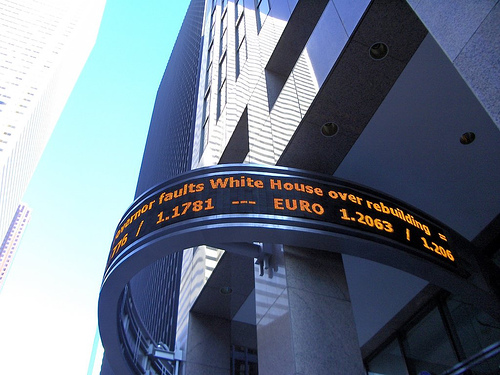
\includegraphics[height=0.50\textheight]{ch1_reuters_ticker.jpg}\\[1mm]
\imgcap{News ticker on the Reuters building, New York}
\imgcredit{https://commons.wikimedia.org/wiki/File:Reuters_News_Ticker.jpg}{Photo: bgilliard (2005); CC BY-SA 2.0; Wikimedia Commons}
\end{column}
\end{columns}
\end{frame}

\begin{frame}{Data Frequency}
\itemsize{\small}
\begin{itemize}
    \item \textbf{Tick data}: every trade and quote
    \begin{itemize}
        \item millions of records per day; noise from the bid--ask bounce
    \end{itemize}
    \item \textbf{Intraday bars}: 1, 5 or 60 minutes
    \begin{itemize}
        \item used for realised volatility (\sfmchlink{https://danpele.github.io/SFM/EN/Courses/chapter8_volatility_estimators.pdf}{Chapter 8})
    \end{itemize}
    \item \textbf{Daily data}: one row per trading day
    \begin{itemize}
        \item the standard of this course and of most academic studies
        \item exchanges trade about 250 days a year; crypto markets trade 365 days a year
    \end{itemize}
    \item \textbf{Weekly, monthly, yearly data}
    \begin{itemize}
        \item fewer observations, closer to the horizon of long-term investors
    \end{itemize}
    \item Rule: annualise with the \textbf{actual} number of observations per year of each series
\end{itemize}
\end{frame}

\begin{frame}{Where the Data Come From}
\itemsize{\small}
\begin{center}
\footnotesize
\begin{tabular}{>{\raggedright\arraybackslash}p{3.4cm}>{\raggedright\arraybackslash}p{5.6cm}>{\raggedright\arraybackslash}p{3.4cm}}
\toprule
\textbf{Source} & \textbf{What it provides} & \textbf{Access} \\
\midrule
Exchanges (BVB, Deutsche Börse, NYSE) & official prices, volumes, index levels & website, paid feeds \\
Data vendors (Bloomberg, LSEG, EODHD) & prices from many venues, adjusted prices, fundamentals & subscription \\
Central banks (BNR, ECB, Federal Reserve) & reference exchange rates, interest rates & free \\
Statistical databases (FRED, Eurostat) & macro series, yields & free \\
Academic databases (CRSP, Kenneth French library) & cleaned returns, including delisted firms; factor returns & university licence or free \\
Crypto exchanges and aggregators & prices 24/7, on-chain data & free or subscription \\
\bottomrule
\end{tabular}
\end{center}
\begin{itemize}
    \item A vendor collects and cleans; the \textbf{primary source} of a number (exchange, central bank) is the reference when two sources disagree
\end{itemize}
\end{frame}

\begin{frame}{The Data of This Course}
\itemsize{\small}
\begin{itemize}
    \item Daily market data from \textbf{EODHD} (EOD Historical Data), saved once in the course repository
    \begin{itemize}
        \item 91 series: indices, ETFs, stocks (BVB, US, Europe), crypto, exchange rates, bond yields
        \item columns: date, open, high, low, close, adjusted close, volume
    \end{itemize}
    \item EUR/RON: the official \textbf{BNR} reference rate
    \begin{itemize}
        \item the EUR/RON series from EODHD has erroneous quotes (next slides)
    \end{itemize}
    \item Conventions
    \begin{itemize}
        \item indices, exchange rates, crypto: \textit{close}; stocks and ETFs: \textit{adjusted close}
        \item weekend quotes and repeated holiday closes are dropped, except for crypto
        \item each series is analysed on its own calendar
    \end{itemize}
    \item Comparison period of the chapter: 1 January 2015 to 18 September 2026
\end{itemize}
\end{frame}

\begin{frame}{Daily Bars: OHLCV}
\itemsize{\footnotesize}
\begin{itemize}
    \item \textbf{OHLCV}: open $O_t$, high $H_t$, low $L_t$, close $C_t$, volume $V_t$ of day $t$
    \item By construction $L_t \le O_t, C_t \le H_t$; the range $H_t - L_t$ measures the intraday spread of prices
    \item Banca Transilvania (TLV), the last five trading days in our data:
\end{itemize}\begin{center}
\footnotesize
\begin{tabular}{lrrrrr}
\toprule
Date & Open & High & Low & Close & Volume \\
\midrule
14 Sep 2026 & $34.52$ & $34.86$ & $34.28$ & $34.54$ & 346\,819 \\
15 Sep 2026 & $34.40$ & $34.68$ & $33.10$ & $34.00$ & 676\,653 \\
16 Sep 2026 & $34.00$ & $34.10$ & $33.20$ & $33.40$ & 853\,078 \\
17 Sep 2026 & $33.40$ & $33.40$ & $33.40$ & $33.40$ & 1\,084\,380 \\
18 Sep 2026 & $34.22$ & $35.80$ & $34.22$ & $35.50$ & 1\,884\,988 \\
\bottomrule
\end{tabular}
\end{center}
\begin{itemize}
    \item Check: on 17 September 2026 open = high = low = close with 1\,084\,380 shares traded; a flat bar with a large volume is suspicious
\end{itemize}
\end{frame}

\begin{frame}{Corporate Actions and the Adjusted Close}
\itemsize{\small}
\begin{itemize}
    \item The traded close $P_t$ jumps on the day of a corporate action; the value of a holding does not
    \item \textbf{Adjustment factor} $A$ on the event day
    \begin{itemize}
        \item cash dividend $D$: $A = 1 - D/P_{t-1}$
        \item split $m$-for-$n$ ($m$ new shares for $n$ old): $A = n/m$; a consolidation is a split with $m < n$
    \end{itemize}
    \item \textbf{Adjusted close}: every earlier price is multiplied by the factors of all later events, $P^{\text{adj}}_t = P_t \prod_{k:\, t_k > t} A_{t_k}$
    \item Returns computed from adjusted prices include the dividend and have no artificial jumps
    \item With dividends, the simple return is $R_t = (P_t + D_t)/P_{t-1} - 1$ \refFHH
\end{itemize}
\end{frame}

\begin{frame}{Worked Example: Adjusted Prices}
\itemsize{\small}
\begin{itemize}
    \item A share trades at 100; on day 5 it pays a cash dividend of 2; on day 10 it splits 2-for-1
    \item Adjustment factors
    \begin{itemize}
        \item dividend: $A_5 = 1 - 2/100 = 0.98$; split: $A_{10} = 1/2 = 0.50$
    \end{itemize}
    \item Adjusted prices
    \begin{itemize}
        \item before day 5: $P^{\text{adj}}_t = P_t \times 0.49$, so 100 becomes 49
        \item between days 5 and 9: $P^{\text{adj}}_t = P_t \times 0.50$; from day 10: $P^{\text{adj}}_t = P_t$
    \end{itemize}
    \item The adjusted series changes every time a new event happens: always keep the download date
    \item Indices: a \textbf{price index} ignores dividends; a \textbf{total return index} reinvests them
\end{itemize}
\end{frame}

\begin{frame}{Real Data: Banca Transilvania, Close vs Adjusted Close}
\itemsize{\footnotesize}
\begin{center}
    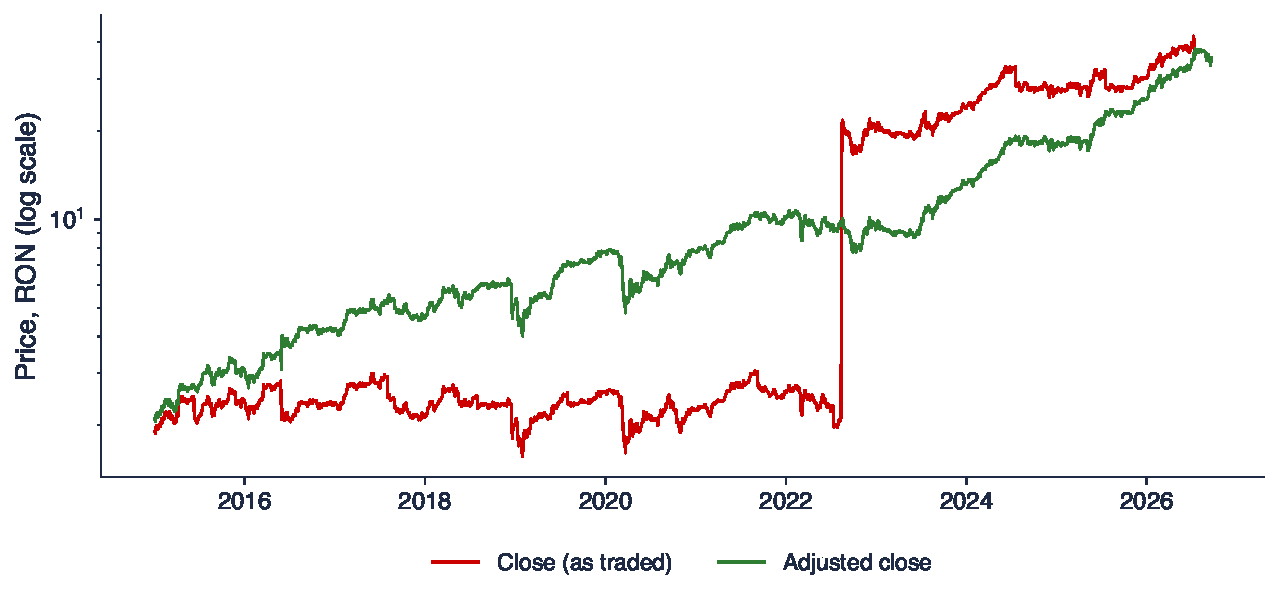
\includegraphics[width=0.97\textwidth,height=0.58\textheight,keepaspectratio]{sfm_ch1_tlv_adjusted.pdf}
\end{center}
\vspace{-0.25cm}
\begin{itemize}
    \item On 16 August 2022 the close jumps from 2.12 to 21.20 RON: a share consolidation, 10 old shares into one
    \item Log return from the close: $+230\%$ in one day; from the adjusted close: $0.0\%$
    \item Since 2015 the two series disagree by more than 2\% on 24 days (dividends, bonus shares)
\end{itemize}
\quantlet{SFM\_ch1\_data\_quality}{\qlurl{SFM_ch1_data_quality}}
\end{frame}

\begin{frame}{Dividends Matter: BET vs BET-TR}
\itemsize{\footnotesize}
\begin{center}
    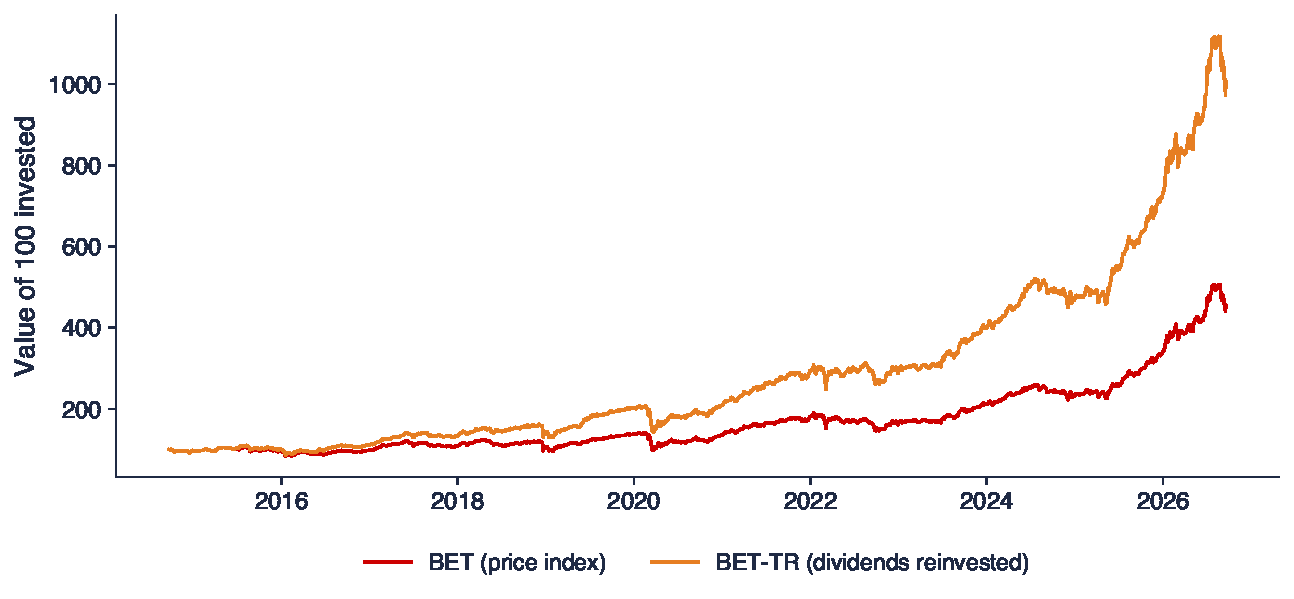
\includegraphics[width=0.97\textwidth,height=0.58\textheight,keepaspectratio]{sfm_ch1_bet_bettr.pdf}
\end{center}
\vspace{-0.25cm}
\begin{itemize}
    \item 100 invested on 23 September 2014: 455 in the BET (price index), 1\,005 in the BET-TR (dividends reinvested)
    \item Growth rate: 13.5\% vs 21.2\% a year; dividends add 7.8 percentage points a year
    \item Compare like with like: the DAX is a total return index, the S\&P 500 and the BET are price indices
\end{itemize}
\quantlet{SFM\_ch1\_data\_quality}{\qlurl{SFM_ch1_data_quality}}
\end{frame}

\begin{frame}{Data Errors: Two EUR/RON Series}
\itemsize{\footnotesize}
\begin{center}
    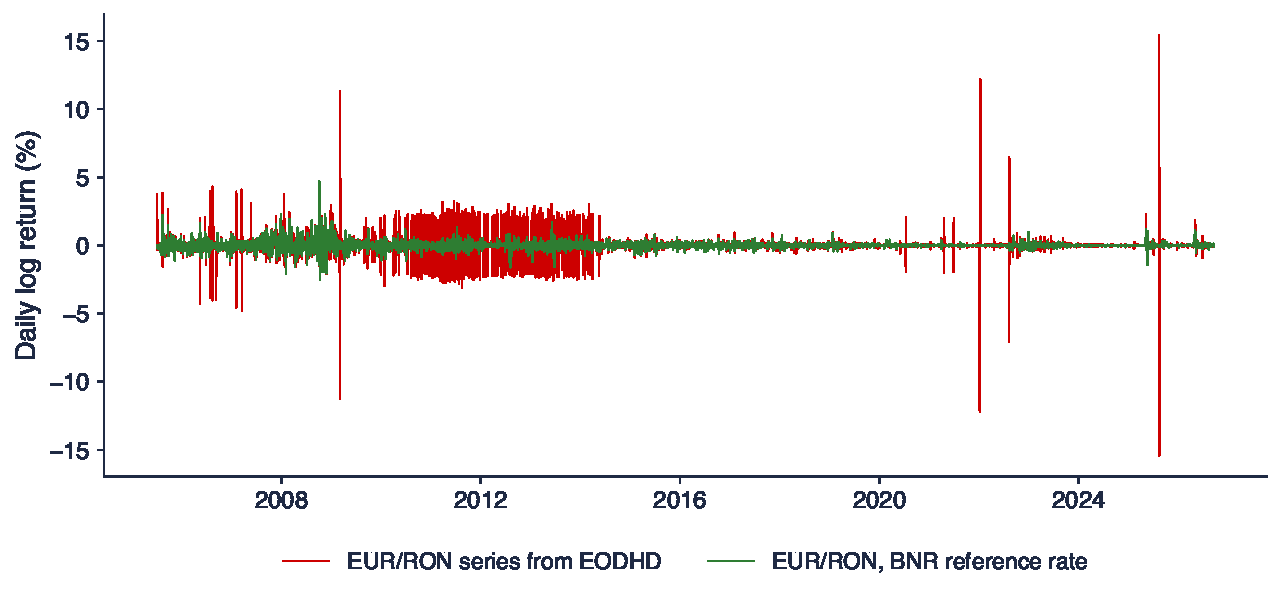
\includegraphics[width=0.97\textwidth,height=0.54\textheight,keepaspectratio]{sfm_ch1_eurron_check.pdf}
\end{center}
\vspace{-0.25cm}
\begin{itemize}
    \item Same exchange rate, 5\,154 common days: the EODHD series moves by more than 1 percentage point more than the BNR rate on 412 days
    \item Annualised volatility: 13.4\% (EODHD) vs 4.5\% (BNR); largest EODHD move $15.4\%$ on 14 August 2025
    \item Fix: use the primary source of the number, the BNR reference rate
\end{itemize}
\quantlet{SFM\_ch1\_data\_quality}{\qlurl{SFM_ch1_data_quality}}
\end{frame}

\begin{frame}{Three Biases That Make Results Look Too Good}
\itemsize{\small}
\begin{itemize}
    \item \textbf{Survivorship bias}: only firms or funds that still exist are in the sample
    \begin{itemize}
        \item the losers have disappeared, so the average return is too high \refBGIR
        \item example: today's members of the BET, followed back to 2000
    \end{itemize}
    \item \textbf{Look-ahead bias}: using information not yet available at the decision date
    \begin{itemize}
        \item annual reports published in March used for decisions in January
    \end{itemize}
    \item \textbf{Data snooping}: trying many rules on the same data and reporting the best one
    \begin{itemize}
        \item hundreds of published return predictors are likely false discoveries \refHLZ
    \end{itemize}
    \item Each bias inflates returns; none shows up in the summary statistics
\end{itemize}
\end{frame}

\begin{frame}{A Data Checklist}
\itemsize{\small}
\begin{itemize}
    \item Source: the primary source of the number and the column used (close or adjusted close)
    \item Calendar: weekends, holidays, missing days; same dates for all assets in a joint analysis
    \item Jumps: list the 10 largest absolute returns and check each against the news
    \item Flat bars, zero volume, repeated prices: holidays filled with the last price or stale quotes
    \item Units and currency: RON, EUR, USD; index points; prices in cents
    \item Keep the raw file and the download date; never edit data manually
\end{itemize}
\end{frame}

\begin{frame}{Recap: Data}
\itemsize{\small}
\begin{itemize}
    \item Prices come from exchanges, vendors and central banks; the primary source of a number is the reference
    \item Use adjusted prices for stocks, total return indices when dividends matter
    \item Real data contain errors: check jumps, flat bars and a second source
    \item Survivorship, look-ahead and data snooping inflate results silently
\end{itemize}
\end{frame}


%=============================================================================
\section{From Prices to Returns}
%=============================================================================

\begin{frame}{Why Returns, Not Prices?}
\itemsize{\small}
\begin{itemize}
    \item A price has a unit and a scale; a return does not
    \begin{itemize}
        \item a 1-leu move is large for a 2-leu share and small for a 500-leu share
    \end{itemize}
    \item Returns of different assets, currencies and periods can be compared directly
    \item Prices trend and wander; returns fluctuate around a stable level
    \begin{itemize}
        \item \textbf{weakly stationary} series: constant mean, constant variance, and a covariance that depends only on the lag
        \item most statistical methods of this course assume (at least) weak stationarity
    \end{itemize}
    \item The investor cares about the relative change of wealth, which is exactly a return
\end{itemize}
\end{frame}

\begin{frame}{S\&P 500: Price Level vs Daily Returns}
\itemsize{\footnotesize}
\begin{center}
    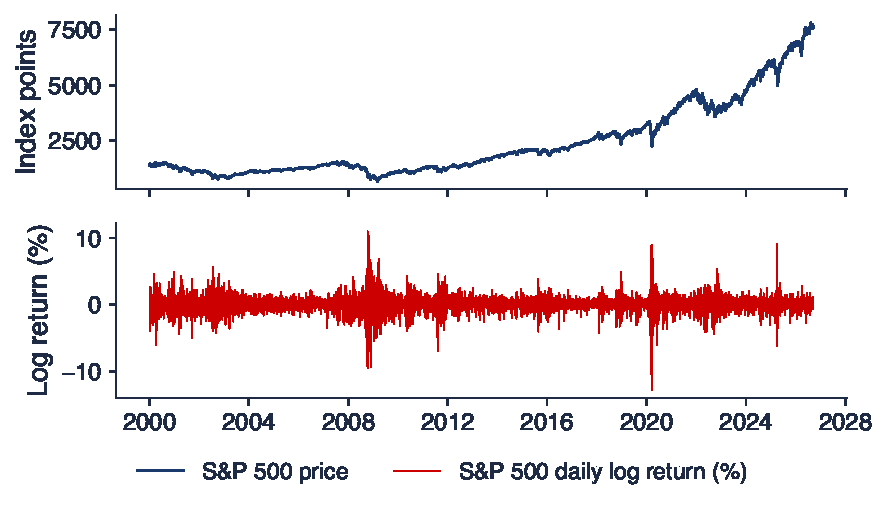
\includegraphics[width=0.97\textwidth,height=0.62\textheight,keepaspectratio]{sfm_ch1_price_returns.pdf}
\end{center}
\vspace{-0.25cm}
\begin{itemize}
    \item Top: the price trends upward with long swings; its mean and spread change over time
    \item Bottom: the returns fluctuate around zero, in calm and turbulent periods (2008, 2020)
\end{itemize}
\quantlet{SFM\_ch1\_prices\_returns}{\qlurl{SFM_ch1_prices_returns}}
\end{frame}

\begin{frame}{A Formal Check: the ADF Test}
\itemsize{\small}
\begin{itemize}
    \item \textbf{ADF test} \refDF: is there a unit root (a random walk) in the series?
    \begin{itemize}
        \item $H_0$: unit root, non-stationary; $H_1$: stationary
        \item regression $\Delta y_t = \alpha + \beta t + \gamma y_{t-1} + \sum_j \delta_j \Delta y_{t-j} + \varepsilon_t$; reject $H_0$ when the $t$-statistic of $\gamma$ is very negative
    \end{itemize}
    \item S\&P 500, daily data since 2000
    \begin{itemize}
        \item log price (with trend): statistic $-2.08$, 5\% critical value $-3.41$, $p = 0.56$: we do not reject the unit root
        \item log returns: statistic $-14.3$, 5\% critical value $-2.86$, $p < 0.001$: we reject it
    \end{itemize}
    \item Unit roots and random walks are the subject of \sfmchlink{https://danpele.github.io/SFM/EN/Courses/chapter7_efficient_markets_random_walk_vr.pdf}{Chapter 7}
\end{itemize}\quantlet{SFM\_ch1\_prices\_returns}{\qlurl{SFM_ch1_prices_returns}}
\end{frame}


%=============================================================================
\section{Simple and Log Returns}
%=============================================================================

\begin{frame}{The Simple Return}
\itemsize{\small}
\begin{itemize}
    \item \textbf{Simple (net) return} from $t-1$ to $t$ \refFHH, \refTsay
    \begin{itemize}
        \item $R_t = \dfrac{P_t - P_{t-1}}{P_{t-1}} = \dfrac{P_t}{P_{t-1}} - 1$
        \item \textbf{gross return}: $1 + R_t = P_t / P_{t-1}$
    \end{itemize}
    \item Bounded below: $R_t \ge -1$ (limited liability: you cannot lose more than you invested)
    \item Example: $P_{t-1} = 100$, $P_t = 110$: $R_t = 10\%$
    \item It is what an investor sees on the account statement: ``the fund gained 10\%''
    \item Notation: from here on $P_t$ is the close of an index or the adjusted close of a stock
\end{itemize}
\end{frame}

\begin{frame}{The Log Return}
\itemsize{\small}
\begin{itemize}
    \item \textbf{Log return} (continuously compounded return)
    \begin{itemize}
        \item $r_t = \ln\dfrac{P_t}{P_{t-1}} = \ln P_t - \ln P_{t-1} = \ln(1 + R_t)$
        \item back to the simple return: $R_t = e^{r_t} - 1$
    \end{itemize}
    \item Name: $e^{r}$ is the growth of 1 leu at rate $r$ compounded continuously over the period
    \item Unbounded: $r_t \in (-\infty, +\infty)$; a total loss ($P_t = 0$) is $r_t = -\infty$
    \item Example: $P_{t-1} = 100$, $P_t = 110$: $r_t = \ln 1.1 = 9.53\%$
    \item Log returns are the default in statistics of financial markets: they add up over time (next section)
\end{itemize}
\end{frame}

\begin{frame}{How Far Apart Are $r$ and $R$?}
\itemsize{\small}
\begin{itemize}
    \item Taylor expansion of the logarithm around 0
    \begin{itemize}
        \item $r = \ln(1 + R) = R - \dfrac{R^2}{2} + \dfrac{R^3}{3} - \dots$
        \item $\ln$ is concave, so $r < R$ for every $R \neq 0$
    \end{itemize}
    \item Daily move, $R = 1\%$
    \begin{itemize}
        \item $r = 0.995\%$, and $R - R^2/2 = 0.995\%$: the gap $R - r$ is 0.5 basis points
    \end{itemize}
    \item Large move, $R = 10\%$
    \begin{itemize}
        \item $r = 9.531\%$, and $R - R^2/2 = 9.500\%$: the gap $R - r$ is 46.9 basis points
    \end{itemize}
    \item A \textbf{basis point} (bp) is 0.01 percentage points
    \item Conclusion: for daily returns $r \approx R$; for large moves and long horizons they differ
\end{itemize}
\end{frame}

\begin{frame}{Simple vs Log Returns on Real Extremes}
\itemsize{\footnotesize}
\begin{columns}[T]
\begin{column}{0.56\textwidth}
\begin{center}
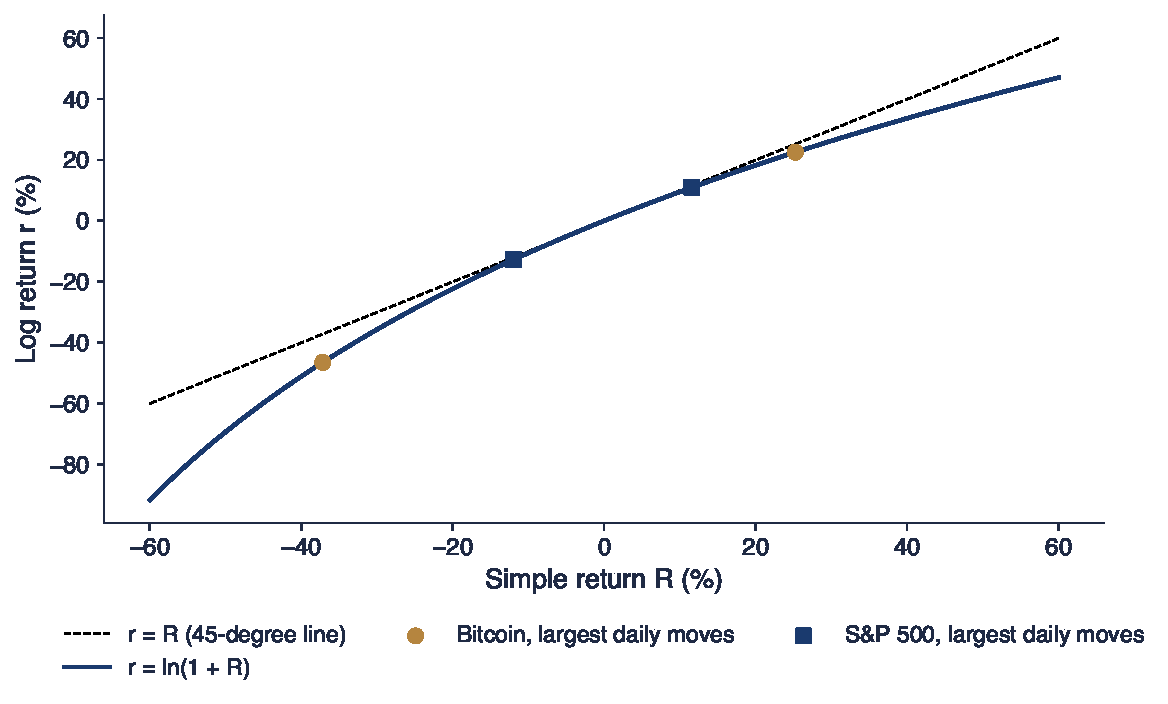
\includegraphics[width=\linewidth,height=0.80\textheight,keepaspectratio]{sfm_ch1_simple_log.pdf}
\end{center}
\end{column}
\begin{column}{0.40\textwidth}
\begin{itemize}
    \item Bitcoin, 12 March 2020: $R = -37.2\%$ but $r = -46.5\%$
    \item Bitcoin, 7 December 2017: $R = +25.2\%$, $r = +22.5\%$
    \item S\&P 500, 16 March 2020: $R = -12.0\%$, $r = -12.8\%$
    \item The curve bends down: losses look larger and gains smaller in log returns
\end{itemize}
\end{column}
\end{columns}
\quantlet{SFM\_ch1\_simple\_log\_returns}{\qlurl{SFM_ch1_simple_log_returns}}
\end{frame}

\begin{frame}{Worked Example: Up 10\%, Then Down 10\%}
\itemsize{\small}
\begin{columns}[T]
\begin{column}{0.58\textwidth}
\begin{itemize}
    \item Price path $100 \to 110 \to 99$
    \begin{itemize}
        \item simple returns: $+10\%$ and $-10\%$; their sum, 0, is misleading
        \item compounded: $1.1 \times 0.9 - 1 = -1.0\%$
    \end{itemize}
    \item Log returns
    \begin{itemize}
        \item $r_1 = \ln 1.1 = 9.53\%$, $r_2 = \ln 0.9 = -10.54\%$
        \item sum: $-1.01\% = \ln(99/100)$, exact
    \end{itemize}
\end{itemize}
\end{column}
\begin{column}{0.38\textwidth}
\begin{block}{Rule}
\begin{itemize}
    \item Simple returns compound (multiply); log returns add
\end{itemize}
\end{block}
\end{column}
\end{columns}
\end{frame}

\begin{frame}{Question for the Room: Up 50\%, Down 50\%}
\itemsize{\small}
\begin{itemize}
    \item A share gains 50\% one year and loses 50\% the next
    \item \textbf{What do you think?} Where is the price after two years, relative to the start?
    \item \textbf{Answer}
    \begin{itemize}
        \item $1.5 \times 0.5 = 0.75$: the wealth changed by $-25\%$
        \item log returns: $\ln 1.5 + \ln 0.5 = \ln 0.75 = -28.8\%$
        \item a loss of $x$ needs a gain of $x/(1-x)$ to recover: 50\% needs 100\%
    \end{itemize}
\end{itemize}
\end{frame}

\begin{frame}{Which Return When?}
\itemsize{\small}
\begin{center}
\footnotesize
\begin{tabular}{>{\raggedright\arraybackslash}p{4.2cm}>{\raggedright\arraybackslash}p{2.6cm}>{\raggedright\arraybackslash}p{5.6cm}}
\toprule
\textbf{Task} & \textbf{Use} & \textbf{Reason} \\
\midrule
Aggregating over time & log & $r_{t}(k) = r_t + \dots + r_{t-k+1}$, a sum \\
Portfolio of several assets & simple & $R_p = \sum_i w_i R_i$, exact \\
Statistical modelling & log & unbounded, closer to a symmetric distribution \\
Reporting to investors & simple & ``the fund gained 10\%'' is a simple return \\
Daily data, small moves & either & the difference is about $R^2/2$ \\
\bottomrule
\end{tabular}
\end{center}
\begin{itemize}
    \item Always say which one you use: a ``return of 10\%'' is ambiguous
\end{itemize}
\end{frame}

\begin{frame}{Recap: Simple and Log Returns}
\itemsize{\small}
\begin{itemize}
    \item $R_t = P_t/P_{t-1} - 1$; $r_t = \ln(P_t/P_{t-1}) = \ln(1 + R_t)$
    \item $r < R$ for every move; the gap is about $R^2/2$, negligible for daily data
    \item Log returns add over time; simple returns add across assets
    \item Gains and losses of the same size do not cancel
\end{itemize}
\end{frame}


%=============================================================================
\section{Multi-Period and Portfolio Returns}
%=============================================================================

\begin{frame}{Returns over $k$ Periods}
\itemsize{\small}
\begin{itemize}
    \item \textbf{Simple}: gross returns multiply
    \begin{itemize}
        \item $1 + R_t(k) = \dfrac{P_t}{P_{t-k}} = (1 + R_t)(1 + R_{t-1}) \cdots (1 + R_{t-k+1})$
    \end{itemize}
    \item \textbf{Log}: returns add
    \begin{itemize}
        \item $r_t(k) = \ln\dfrac{P_t}{P_{t-k}} = r_t + r_{t-1} + \dots + r_{t-k+1}$
    \end{itemize}
    \item Consequence: the mean and variance of a $k$-day log return follow from those of the daily returns
    \item Weekly, monthly or yearly returns are computed from the prices at the end of each period, not by averaging
\end{itemize}
\end{frame}

\begin{frame}{Cumulative Return and Wealth}
\itemsize{\small}
\begin{itemize}
    \item Wealth after $T$ periods, starting from $W_0$: $W_T = W_0 \prod_{t=1}^{T} (1 + R_t) = W_0 \exp\Big(\sum_{t=1}^{T} r_t\Big)$
    \item \textbf{Cumulative simple return}: $\text{CSR}_T = W_T/W_0 - 1$
    \begin{itemize}
        \item what the investor gained, in percent
    \end{itemize}
    \item \textbf{Cumulative log return}: $\text{CLR}_T = \ln(W_T/W_0) = \sum_t r_t$
    \begin{itemize}
        \item link: $\text{CSR}_T = e^{\text{CLR}_T} - 1$
    \end{itemize}
    \item Log scale on charts: equal vertical distances are equal percentage changes
\end{itemize}
\end{frame}

\begin{frame}{Growth of 100 Invested, 2015--2026}
\itemsize{\footnotesize}
\begin{center}
    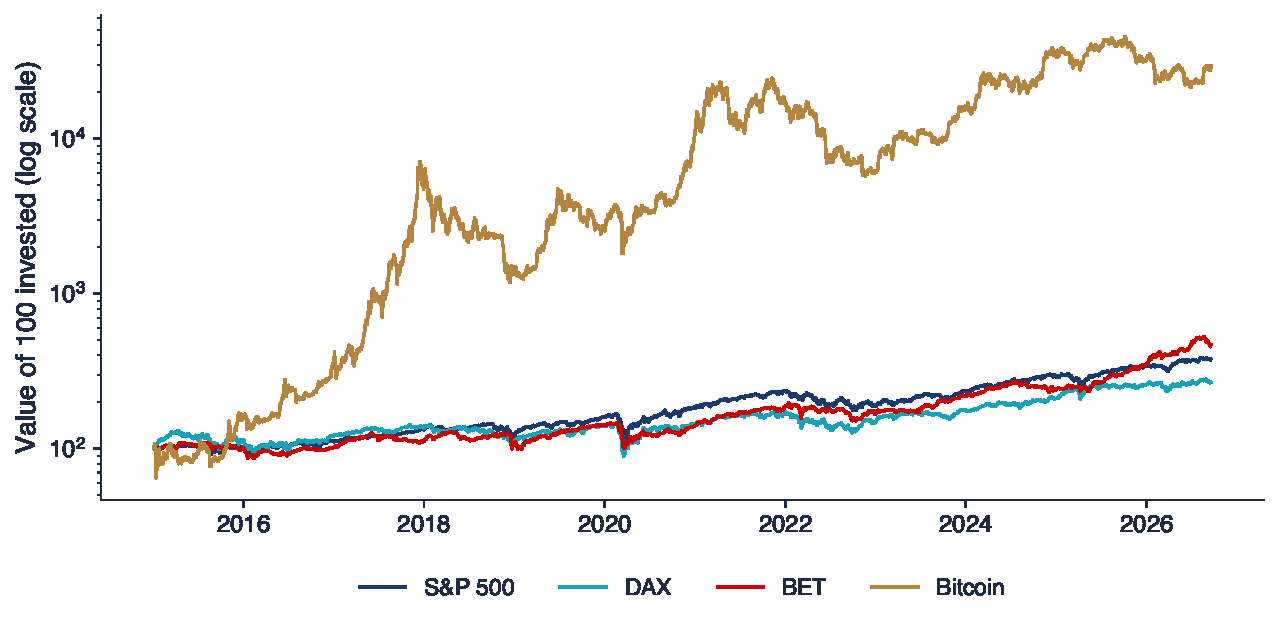
\includegraphics[width=0.97\textwidth,height=0.58\textheight,keepaspectratio]{sfm_ch1_growth.pdf}
\end{center}
\vspace{-0.25cm}
\begin{itemize}
    \item Final values: S\&P 500 379, DAX 267, BET 470, Bitcoin 29\,475
    \item Bitcoin: cumulative simple return 29\,375\%, cumulative log return 5.69; BET: 370\% and 1.55
    \item Without the log scale, every series except Bitcoin would look flat
\end{itemize}
\quantlet{SFM\_ch1\_portfolio\_returns}{\qlurl{SFM_ch1_portfolio_returns}}
\end{frame}

\begin{frame}{Portfolio Returns}
\itemsize{\small}
\begin{itemize}
    \item Portfolio with weights $w_1, \dots, w_n$, $\sum_i w_i = 1$, set at the start of the period
    \begin{itemize}
        \item \textbf{simple}: $R_p = \sum_i w_i R_i$, exact
        \item \textbf{log}: $r_p = \ln\big(\sum_i w_i e^{r_i}\big) \neq \sum_i w_i r_i$
    \end{itemize}
    \item Example: 60\% in A ($R_A = 10\%$), 40\% in B ($R_B = -5\%$)
    \begin{itemize}
        \item $R_p = 0.6 \times 10\% + 0.4 \times (-5\%) = 4.0\%$; exact $r_p = \ln(1 + R_p) = 3.92\%$
        \item weighted log returns: $0.6 \times 9.53\% + 0.4 \times (-5.13\%) = 3.67\%$, too low
    \end{itemize}
    \item Weights drift when prices move: a fixed-weight portfolio must be \textbf{rebalanced}
\end{itemize}\quantlet{SFM\_ch1\_portfolio\_returns}{\qlurl{SFM_ch1_portfolio_returns}}
\end{frame}

\begin{frame}{Real Data: a TLV--SNP Portfolio}
\itemsize{\small}
\begin{itemize}
    \item 50\% Banca Transilvania, 50\% OMV Petrom, rebalanced daily, 2015--2026
    \item One day: exact log return vs weighted sum of log returns
    \begin{itemize}
        \item mean absolute gap 0.38 basis points; largest gap 13.9 basis points, on 31 May 2016
    \end{itemize}
    \item Over the whole period the small gaps accumulate
    \begin{itemize}
        \item exact cumulative log return 2.56, so 1 leu grows to 13.0 lei
        \item weighted log returns give 2.47, so only 11.8 lei
    \end{itemize}
    \item Growth rate: portfolio 24.5\% a year; TLV 27.3\%; SNP 19.7\%
    \item Rule: build portfolios with simple returns, then take logs if needed
\end{itemize}\quantlet{SFM\_ch1\_portfolio\_returns}{\qlurl{SFM_ch1_portfolio_returns}}
\end{frame}

\begin{frame}{Recap: Multi-Period and Portfolio Returns}
\itemsize{\small}
\begin{itemize}
    \item Over time: multiply gross returns or add log returns
    \item Wealth $W_T = W_0 e^{\text{CLR}_T}$; $\text{CSR}_T = e^{\text{CLR}_T} - 1$
    \item Across assets: $R_p = \sum_i w_i R_i$ exactly; the log version is only an approximation
    \item Small daily approximation errors become visible over a decade
\end{itemize}
\end{frame}


%=============================================================================
\section{Annualisation}
%=============================================================================

\begin{frame}{Annualising the Mean and the Volatility}
\itemsize{\small}
\begin{itemize}
    \item $q$ = number of observations per year: about 252 for exchanges, 365 for crypto, 52 for weekly, 12 for monthly data
    \item \textbf{Mean}: log returns add, so $\mu_{\text{year}} = q\,\mu$
    \begin{itemize}
        \item the same rule is used for the mean of simple returns (arithmetic annualisation)
    \end{itemize}
    \item \textbf{Volatility} = standard deviation of returns: $\sigma_{\text{year}} = \sqrt{q}\,\sigma$, the \textbf{square-root-of-time rule}
    \begin{itemize}
        \item valid when returns are uncorrelated with constant variance: then $\Var(r_1 + \dots + r_q) = q\,\sigma^2$
    \end{itemize}
    \item S\&P 500: daily $\sigma = 1.12\%$, so $\sigma_{\text{year}} = 1.12\% \times 15.87 = 17.7\%$
    \begin{itemize}
        \item Bitcoin: $\sqrt{365} = 19.10$ gives 66.6\%; the stock-market factor $\sqrt{252}$ would give only 55.4\%
    \end{itemize}
\end{itemize}
\end{frame}

\begin{frame}{The Compound Annual Growth Rate}
\itemsize{\small}
\begin{itemize}
    \item \textbf{CAGR} (compound annual growth rate): the constant yearly rate that turns $P_0$ into $P_T$ in $Y$ years
    \begin{itemize}
        \item $\text{CAGR} = \big(P_T / P_0\big)^{1/Y} - 1$, with $Y$ in calendar years
    \end{itemize}
    \item Link with log returns: $\text{CAGR} = \exp(\text{annual mean log return}) - 1$
    \item S\&P 500, 2015--2026: mean log return 11.2\% a year, $e^{11.2\%} - 1 = 11.9\%$, the CAGR is 11.9\%
    \item The CAGR uses only the first and the last price: it says nothing about the path in between
    \item Also called the geometric mean return
\end{itemize}
\end{frame}

\begin{frame}{How Precisely Do We Know the Mean?}
\itemsize{\small}
\begin{itemize}
    \item Standard error of the annual mean: $\text{SE}(\hat\mu_{\text{year}}) = \sigma_{\text{year}} / \sqrt{Y}$, with $Y$ years of data
    \begin{itemize}
        \item it depends on the number of \textbf{years}, not on the number of observations
    \end{itemize}
    \item S\&P 500, 11.7 years: annual mean log return 11.2\%, SE 5.2\%
    \begin{itemize}
        \item 95\% CI (confidence interval): [1.1\%, 21.4\%]
    \end{itemize}
    \item Bitcoin: 47.4\% $\pm$ $1.96 \times 19.5\%$
    \begin{itemize}
        \item the interval is [9.2\%, 85.6\%]: very wide
    \end{itemize}
    \item Volatility, by contrast, is estimated precisely from daily data
\end{itemize}\quantlet{SFM\_ch1\_descriptive\_stats}{\qlurl{SFM_ch1_descriptive_stats}}
\end{frame}

\begin{frame}{Question for the Room: More Data, Better Mean?}
\itemsize{\small}
\begin{itemize}
    \item You replace 10 years of daily S\&P 500 data by 10 years of 5-minute data: 78 bars in a 6.5-hour trading day, so 78 times more observations
    \item \textbf{What do you think?} Does the standard error of the annual mean return become smaller?
    \item \textbf{Answer}
    \begin{itemize}
        \item No: the mean over 10 years is fixed by the first and last price, $\hat\mu = \ln(P_T/P_0)/Y$
        \item only more \textbf{years} reduce its standard error, as $1/\sqrt{Y}$
        \item the volatility estimate, in contrast, does improve with higher frequency
    \end{itemize}
\end{itemize}
\end{frame}

\begin{frame}{Recap: Annualisation}
\itemsize{\small}
\begin{itemize}
    \item Mean $\times\, q$, volatility $\times \sqrt{q}$, with $q$ the actual observations per year
    \item $\sqrt{q}$ assumes uncorrelated returns with constant variance
    \item CAGR $= (P_T/P_0)^{1/Y} - 1$, the exponential of the annual mean log return minus 1
    \item Mean returns are imprecise: SE $= \sigma_{\text{year}}/\sqrt{Y}$
\end{itemize}
\end{frame}


%=============================================================================
\section{Descriptive Statistics of Returns}
%=============================================================================

\begin{frame}{Location and Spread}
\itemsize{\small}
\begin{itemize}
    \item Sample $r_1, \dots, r_n$ of daily log returns (in \%)
    \item \textbf{Mean}: $\bar r = \frac1n \sum_{t=1}^{n} r_t$, the average daily return
    \item \textbf{Variance}: $\hat\sigma^2 = \frac{1}{n-1} \sum_{t=1}^{n} (r_t - \bar r)^2$; \textbf{standard deviation} $\hat\sigma = \sqrt{\hat\sigma^2}$
    \begin{itemize}
        \item in finance the standard deviation of returns is called \textbf{volatility}
    \end{itemize}
    \item \textbf{Quantile} $q_\alpha$: the value below which a fraction $\alpha$ of returns lie
    \begin{itemize}
        \item median $q_{0.5}$; the 1\% quantile $q_{0.01}$ is the basis of VaR 1\% (Chapter 10)
    \end{itemize}
    \item \textbf{Minimum} and \textbf{maximum}: the worst and best day, always with their dates
\end{itemize}
\end{frame}

\begin{frame}{Shape: Skewness and Kurtosis}
\itemsize{\small}
\begin{itemize}
    \item \textbf{Skewness}: $\hat S = \frac1n \sum_t (r_t - \bar r)^3 / \hat\sigma^3$
    \begin{itemize}
        \item $S = 0$: symmetric; $S < 0$: a longer left tail, large losses more frequent than large gains
    \end{itemize}
    \item \textbf{Kurtosis}: $\hat K = \frac1n \sum_t (r_t - \bar r)^4 / \hat\sigma^4$; \textbf{excess kurtosis} $\hat K - 3$
    \begin{itemize}
        \item the Normal distribution has $K = 3$, so excess kurtosis 0
        \item excess kurtosis $> 0$: \textbf{heavy tails}, extreme days more frequent than under the Normal distribution
    \end{itemize}
    \item Both are sensitive to single extreme days: report them with the extremes
    \item Heavy tails and asymmetry are \textbf{stylised facts} of returns \refCont; formal tests in \sfmchlink{https://danpele.github.io/SFM/EN/Courses/chapter2_classical_distributions_stylised_facts.pdf}{Chapter 2}
\end{itemize}
\end{frame}

\begin{frame}{Daily Log Returns: Indices and Bitcoin, 2015--2026}
\itemsize{\small}
\begin{center}
\footnotesize
\begin{tabular}{lrrrrlr}
\toprule
Series & Mean & Std. dev. & Skew. & Exc. kurt. & Minimum (date) & Maximum \\
\midrule
S\&P 500 & $0.045$ & $1.12$ & $-0.64$ & $15.8$ & $-12.8$ (16 Mar 2020) & $9.1$ \\
DAX & $0.032$ & $1.20$ & $-0.56$ & $10.0$ & $-13.1$ (12 Mar 2020) & $10.4$ \\
BET & $0.053$ & $0.98$ & $-1.41$ & $17.8$ & $-11.9$ (19 Dec 2018) & $6.8$ \\
BET-TR & $0.080$ & $0.98$ & $-1.43$ & $18.1$ & $-11.9$ (19 Dec 2018) & $6.7$ \\
Bitcoin & $0.130$ & $3.49$ & $-0.73$ & $12.2$ & $-46.5$ (12 Mar 2020) & $22.5$ \\
\bottomrule
\end{tabular}
\end{center}
\begin{itemize}
    \item All values in \% except skewness and excess kurtosis; each series on its own calendar
    \item Bitcoin: daily standard deviation about three times that of the stock indices
    \item All series: negative skewness and large excess kurtosis
    \item The worst days cluster in March 2020 (COVID-19) and on 19 December 2018 for the BET
\end{itemize}\quantlet{SFM\_ch1\_descriptive\_stats}{\qlurl{SFM_ch1_descriptive_stats}}
\end{frame}

\begin{frame}{Daily Log Returns: Five BVB Stocks, 2015--2026}
\itemsize{\small}
\begin{center}
\footnotesize
\begin{tabular}{lrrrrlr}
\toprule
Series & Mean & Std. dev. & Skew. & Exc. kurt. & Minimum (date) & Maximum \\
\midrule
Banca Transilvania (TLV) & $0.106$ & $1.69$ & $-0.55$ & $25.2$ & $-22.2$ (19 Dec 2018) & $20.5$ \\
OMV Petrom (SNP) & $0.079$ & $1.54$ & $-0.66$ & $9.2$ & $-15.0$ (9 Mar 2020) & $10.0$ \\
BRD & $0.075$ & $1.61$ & $-0.51$ & $9.2$ & $-18.2$ (19 Dec 2018) & $10.3$ \\
Nuclearelectrica (SNN) & $0.118$ & $1.53$ & $0.29$ & $5.2$ & $-9.4$ (9 Mar 2020) & $11.3$ \\
Transgaz (TGN) & $0.091$ & $1.55$ & $0.01$ & $5.3$ & $-10.1$ (19 Dec 2018) & $11.1$ \\
\bottomrule
\end{tabular}
\end{center}
\begin{itemize}
    \item Single stocks are more volatile than the BET index: diversification at work
    \item Banca Transilvania and BRD lost most on 19 December 2018, after the announcement of a tax on bank assets, adopted as OUG 114/2018
    \item Excess kurtosis differs widely between stocks: compare TLV with SNN
    \item Crashes on the BVB have their own statistics \refPele
\end{itemize}\quantlet{SFM\_ch1\_descriptive\_stats}{\qlurl{SFM_ch1_descriptive_stats}}
\end{frame}

\begin{frame}{Histograms vs the Normal Distribution}
\itemsize{\footnotesize}
\begin{center}
    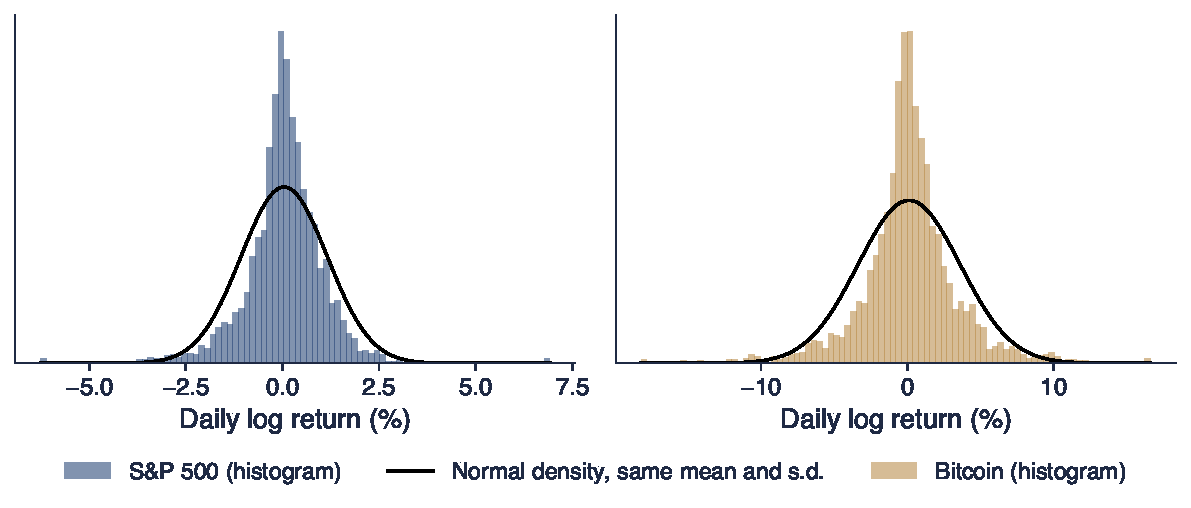
\includegraphics[width=0.97\textwidth,height=0.55\textheight,keepaspectratio]{sfm_ch1_hist_normal.pdf}
\end{center}
\vspace{-0.25cm}
\begin{itemize}
    \item Black line: the Normal density with the same mean and standard deviation
    \item S\&P 500: 79.6\% of days lie within one standard deviation of the mean (Normal: 68.3\%)
    \item Beyond three standard deviations: 1.39\% of days vs 0.27\% under the Normal distribution, 5.2 times more
\end{itemize}
\quantlet{SFM\_ch1\_descriptive\_stats}{\qlurl{SFM_ch1_descriptive_stats}}
\end{frame}

\begin{frame}{Volatility Changes over Time}
\itemsize{\footnotesize}
\begin{center}
    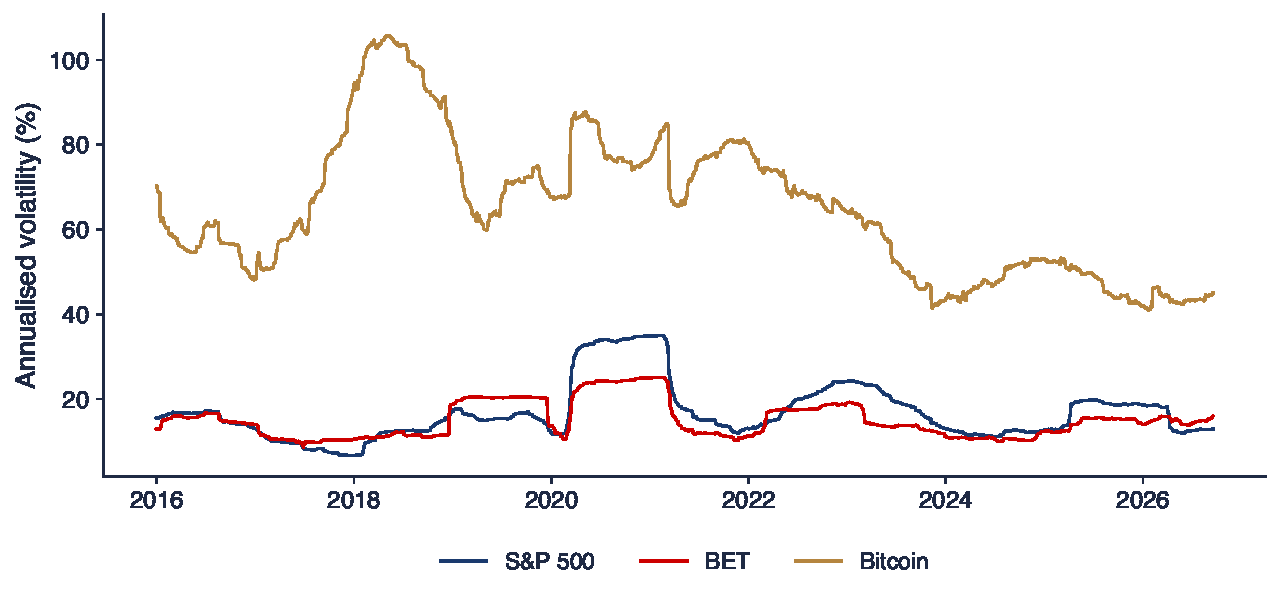
\includegraphics[width=0.97\textwidth,height=0.55\textheight,keepaspectratio]{sfm_ch1_rolling_vol_1y.pdf}
\end{center}
\vspace{-0.25cm}
\begin{itemize}
    \item Rolling one-year volatility, annualised: S\&P 500 between 7\% and 35\%; Bitcoin between 41\% and 106\%
    \item One number for the whole sample hides calm and turbulent periods
    \item Volatility estimators and GARCH models: \sfmchlink{https://danpele.github.io/SFM/EN/Courses/chapter8_volatility_estimators.pdf}{Chapters 8} and \sfmchlink{https://danpele.github.io/SFM/EN/Courses/chapter9_arch_garch_models.pdf}{9}
\end{itemize}
\quantlet{SFM\_ch1\_descriptive\_stats}{\qlurl{SFM_ch1_descriptive_stats}}
\end{frame}

\begin{frame}{Recap: Descriptive Statistics}
\itemsize{\small}
\begin{itemize}
    \item Report mean, standard deviation, skewness, excess kurtosis, quantiles and extremes with dates
    \item Daily returns: mean near 0, volatility 1--3\% a day, heavy tails, often negative skewness
    \item Extreme days are several times more frequent than under the Normal distribution
    \item Volatility is not constant over time
\end{itemize}
\end{frame}


%=============================================================================
\section{Performance Indicators}
%=============================================================================

\begin{frame}{Why One Number Is Not Enough}
\itemsize{\small}
\begin{itemize}
    \item Return alone rewards risk taking: a leveraged bet can show a high return for years
    \item Three questions an investor asks
    \begin{itemize}
        \item how much did it grow? (CAGR)
        \item how bumpy was the ride? (volatility, downside deviation)
        \item how deep was the worst fall? (maximum drawdown)
    \end{itemize}
    \item \textbf{Risk-adjusted} indicators divide a return by a risk measure: Sharpe, Sortino, Calmar
    \item All are estimates from one sample: each has an estimation error
\end{itemize}
\end{frame}

\begin{frame}{The Sharpe Ratio}
\itemsize{\small}
\begin{columns}[T]
\begin{column}{0.64\textwidth}
\begin{itemize}
    \item \textbf{Sharpe ratio} \refSharpeA, \refSharpeB: excess return per unit of total risk
    \begin{itemize}
        \item $\text{SR} = \dfrac{\mu - r_f}{\sigma}$; $\mu$ mean return, $r_f$ risk-free rate, $\sigma$ volatility
        \item from daily to annual: $\text{SR}_{\text{year}} = \sqrt{q}\,\text{SR}_{\text{day}}$
    \end{itemize}
    \item Here: mean of daily simple returns, $r_f = 0$
    \begin{itemize}
        \item the assets are in RON, EUR and USD, each with its own risk-free rate
        \item S\&P 500: daily SR $0.046$, annual SR $0.72$
    \end{itemize}
    \item Same Sharpe ratio, same return per unit of risk, whatever the leverage
\end{itemize}
\end{column}
\begin{column}{0.32\textwidth}
\centering
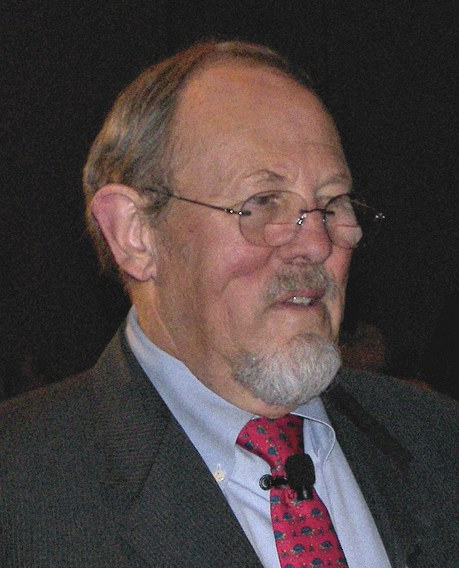
\includegraphics[height=0.55\textheight]{ch1_sharpe_2007.jpg}\\[1mm]
\imgcap{William F. Sharpe, Nobel Prize in Economics 1990}
\imgcredit{https://commons.wikimedia.org/wiki/File:William_sharpe_2007.jpg}{Photo: Larry D. Moore (2007); CC BY 4.0; Wikimedia Commons}
\end{column}
\end{columns}
\end{frame}

\begin{frame}{The Sharpe Ratio Is an Estimate}
\itemsize{\small}
\begin{itemize}
    \item Standard error for i.i.d. (independent, identically distributed) returns \refLo
    \begin{itemize}
        \item $\text{SE}(\widehat{\text{SR}}) \approx \sqrt{(1 + \text{SR}^2/2)/n}$ per period; annual: multiply by $\sqrt{q}$
        \item roughly $1/\sqrt{Y}$ for the annual Sharpe ratio: about $0.3$ with 12 years of data
    \end{itemize}
    \item S\&P 500, 2015--2026: $\text{SR} = 0.72$, SE $0.29$
    \begin{itemize}
        \item 95\% CI [$0.15$, $1.30$]
    \end{itemize}
    \item Heavy tails and volatility clustering make the true error larger than this formula
    \item Choosing the best of many strategies inflates the winner's Sharpe ratio \refDSR
\end{itemize}\quantlet{SFM\_ch1\_performance}{\qlurl{SFM_ch1_performance}}
\end{frame}

\begin{frame}{Sharpe Ratios with 95\% Intervals, 2015--2026}
\itemsize{\footnotesize}
\begin{columns}[T]
\begin{column}{0.58\textwidth}
\begin{center}
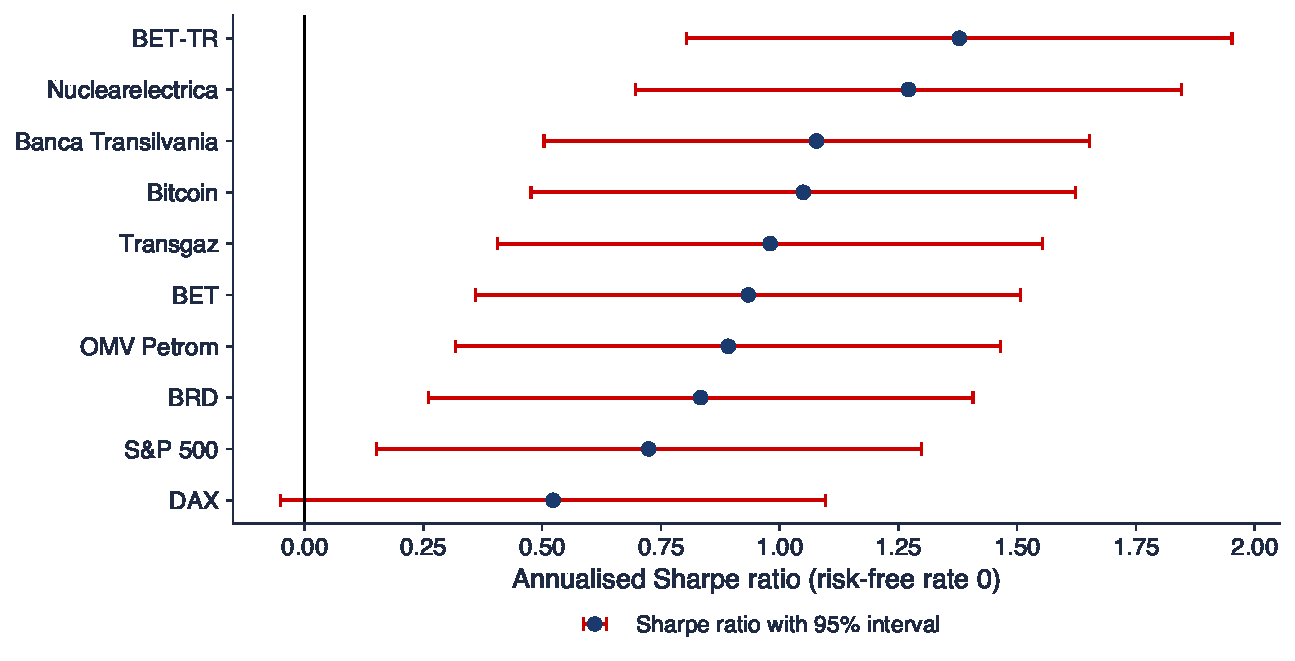
\includegraphics[width=\linewidth,height=0.80\textheight,keepaspectratio]{sfm_ch1_sharpe_ci.pdf}
\end{center}
\end{column}
\begin{column}{0.38\textwidth}
\begin{itemize}
    \item Highest point estimate: BET-TR
    \item All intervals overlap: the ranking is not statistically significant
    \item The DAX interval contains 0
    \item Interval widths are almost equal: they depend mainly on the length of the sample
\end{itemize}
\end{column}
\end{columns}
\quantlet{SFM\_ch1\_performance}{\qlurl{SFM_ch1_performance}}
\end{frame}

\begin{frame}{The Sortino Ratio}
\itemsize{\small}
\begin{itemize}
    \item Investors dislike losses, not gains: the volatility treats both the same
    \item \textbf{Downside deviation} below a target $\tau$ (here $\tau = 0$)
    \begin{itemize}
        \item $\sigma_D = \sqrt{\frac1n \sum_t \min(R_t - \tau, 0)^2}$, only days below the target count
    \end{itemize}
    \item \textbf{Sortino ratio} \refSortino: $\text{Sortino} = \dfrac{\mu - \tau}{\sigma_D}$, annualised like the Sharpe ratio
    \item For a symmetric distribution $\sigma_D \approx \sigma/\sqrt2$, so Sortino $\approx 1.4 \times$ Sharpe
    \item S\&P 500, 2015--2026: Sharpe $0.72$, Sortino $1.02$
\end{itemize}
\end{frame}

\begin{frame}{Drawdown and Maximum Drawdown}
\itemsize{\small}
\begin{itemize}
    \item \textbf{Drawdown}: the fall from the highest price reached so far
    \begin{itemize}
        \item $\text{DD}_t = \dfrac{P_t}{\max_{s \le t} P_s} - 1 \le 0$; zero at a new maximum
    \end{itemize}
    \item \textbf{MDD} (maximum drawdown): $\text{MDD} = \min_t \text{DD}_t$, the worst peak-to-trough fall
    \begin{itemize}
        \item also report the dates: peak, trough and \textbf{recovery} (back to the old peak)
    \end{itemize}
    \item A loss $x$ needs a gain $x/(1 - x)$ to recover
    \begin{itemize}
        \item 10\% needs 11\%; 20\% needs 25\%; 50\% needs 100\%; 80\% needs 400\%
    \end{itemize}
    \item The MDD depends on the path and grows with the length of the sample \refMagdon
\end{itemize}
\end{frame}

\begin{frame}{Drawdowns over the Full History}
\itemsize{\footnotesize}
\begin{center}
    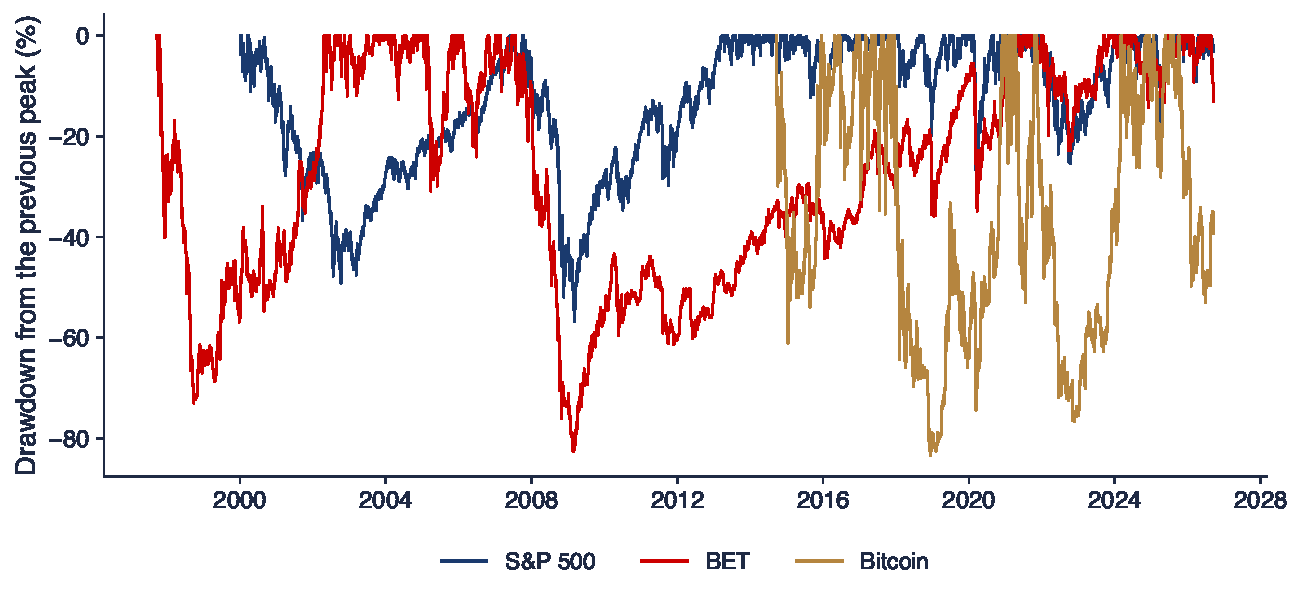
\includegraphics[width=0.97\textwidth,height=0.55\textheight,keepaspectratio]{sfm_ch1_drawdowns.pdf}
\end{center}
\vspace{-0.25cm}
\begin{itemize}
    \item S\&P 500: MDD $-56.8\%$, 9 Oct 2007 to 9 Mar 2009, recovered on 28 Mar 2013
    \item BET (since 1997): MDD $-82.5\%$, 24 Jul 2007 to 25 Feb 2009, recovered only on 16 Mar 2021
    \item Bitcoin: MDD $-83.4\%$, 16 Dec 2017 to 15 Dec 2018
\end{itemize}
\quantlet{SFM\_ch1\_performance}{\qlurl{SFM_ch1_performance}}
\end{frame}

\begin{frame}{Reading the Drawdown Chart}
\itemsize{\small}
\begin{itemize}
    \item Depth
    \begin{itemize}
        \item after a drawdown of $-82.5\%$, the BET needed $+473\%$ to recover; Bitcoin, $+502\%$
    \end{itemize}
    \item Duration
    \begin{itemize}
        \item the BET needed 13.6 years to regain its 2007 peak
        \item share of days more than 20\% below the peak: S\&P 500 27\%, BET 56\%, Bitcoin 66\%
    \end{itemize}
    \item Volatility and Sharpe ratio ignore the order of returns; the drawdown does not
    \item In the comparison period 2015--2026, the MDD of each stock index happened in February--March 2020; Bitcoin and several BVB stocks had theirs at other dates
\end{itemize}
\end{frame}

\begin{frame}{The Calmar Ratio}
\itemsize{\small}
\begin{itemize}
    \item \textbf{Calmar ratio}: growth per unit of the worst fall, $\text{Calmar} = \dfrac{\text{CAGR}}{|\text{MDD}|}$
    \item Popular with fund managers: the MDD is the loss an investor actually lives through
    \item S\&P 500, 2015--2026: CAGR 11.9\%, MDD $-33.9\%$
    \begin{itemize}
        \item Calmar $= 11.9/33.9 = 0.35$
    \end{itemize}
    \item A single event decides the denominator: the Calmar ratio is even noisier than the Sharpe ratio
    \item Compare Calmar ratios only over the same period
\end{itemize}
\end{frame}

\begin{frame}{Volatility Drag}
\itemsize{\small}
\begin{itemize}
    \item For a log return with mean $m$ and variance $\sigma^2$, the simple return has mean $\approx m + \sigma^2/2$
    \begin{itemize}
        \item so the growth rate is $\mu_{\text{log}} \approx \mu_{\text{arith}} - \sigma^2/2$
        \item the gap $\sigma^2/2$ is the \textbf{volatility drag} \refBoothFama; it comes from the concavity of $\ln$ (Jensen's inequality)
    \end{itemize}
    \item Two assets with the same arithmetic mean, 10\% a year
    \begin{itemize}
        \item $\sigma = 5\%$: drag 0.12\%, growth 9.88\% a year; after 10 years 1 leu becomes 2.68
        \item $\sigma = 30\%$: drag 4.50\%, growth 5.50\% a year; after 10 years 1 leu becomes 1.73
    \end{itemize}
    \item Doubling the volatility quadruples the drag
\end{itemize}
\end{frame}

\begin{frame}{Volatility Drag on Real Data}
\itemsize{\footnotesize}
\begin{columns}[T]
\begin{column}{0.56\textwidth}
\begin{center}
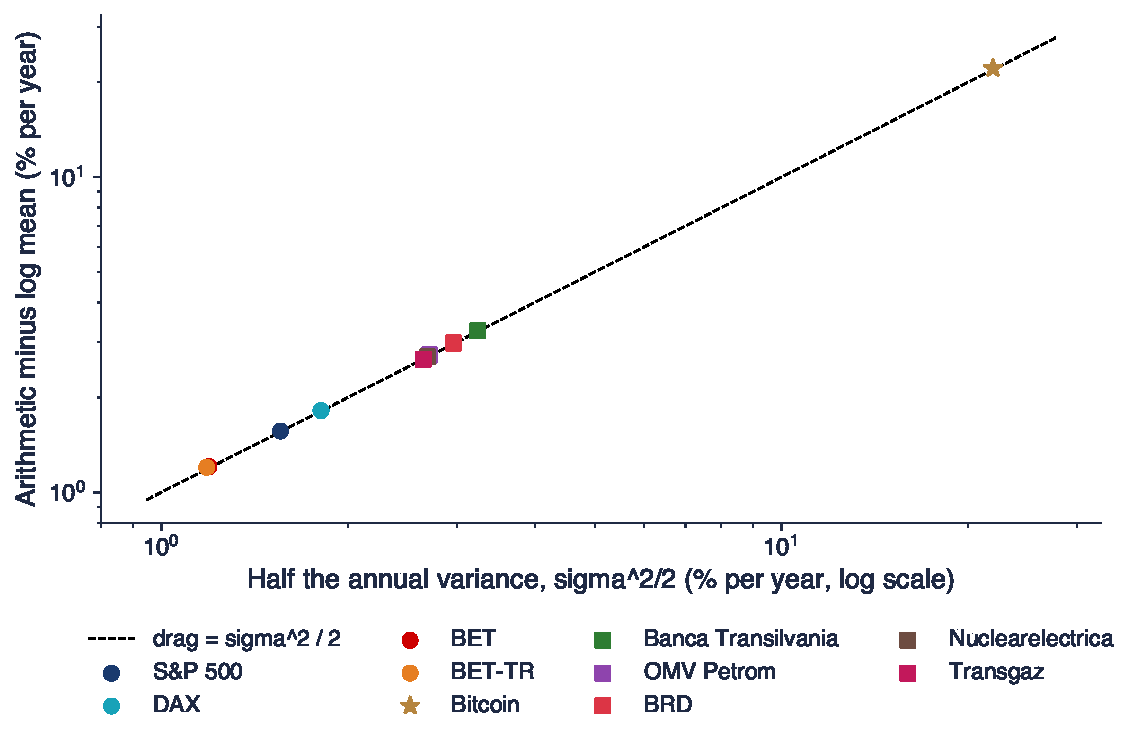
\includegraphics[width=\linewidth,height=0.80\textheight,keepaspectratio]{sfm_ch1_vol_drag.pdf}
\end{center}
\end{column}
\begin{column}{0.40\textwidth}
\begin{itemize}
    \item Each point: one asset, 2015--2026
    \item Vertical: arithmetic minus log annual mean; horizontal: $\sigma^2/2$
    \item All points lie on the line: the formula works on real data
    \item Bitcoin: arithmetic mean 69.5\%, log mean 47.4\%, drag 22.1 percentage points; $\sigma^2/2 = 21.9\%$
\end{itemize}
\end{column}
\end{columns}
\quantlet{SFM\_ch1\_volatility\_drag}{\qlurl{SFM_ch1_volatility_drag}}
\end{frame}

\begin{frame}{Question for the Room: Which Bitcoin Return?}
\itemsize{\small}
\begin{itemize}
    \item Bitcoin, 2015--2026: arithmetic mean of simple returns 69.5\% a year; CAGR 60.6\%
    \item \textbf{What do you think?} Which number describes the growth of an investor's wealth?
    \item \textbf{Answer}
    \begin{itemize}
        \item the CAGR: it is the rate that actually turned the first price into the last
        \item the arithmetic mean is the expected return of a single year, not the growth over many years
        \item the gap is the volatility drag; for low-volatility assets it is small
    \end{itemize}
\end{itemize}
\end{frame}

\begin{frame}{Performance Indicators: Indices and Bitcoin, 2015--2026}
\itemsize{\small}
\begin{center}
\footnotesize
\begin{tabular}{lrrrrrrr}
\toprule
& CAGR \% & Vol. \% & Sharpe & Sortino & MDD \% & Calmar & Drag \% \\
\midrule
S\&P 500 & $11.9$ & $17.6$ & $0.72$ & $1.02$ & $-33.9$ & $0.35$ & $1.56$ \\
DAX & $8.5$ & $19.0$ & $0.52$ & $0.73$ & $-38.8$ & $0.22$ & $1.82$ \\
BET & $14.1$ & $15.4$ & $0.93$ & $1.28$ & $-31.1$ & $0.45$ & $1.21$ \\
BET-TR & $22.1$ & $15.4$ & $1.38$ & $1.92$ & $-31.1$ & $0.71$ & $1.20$ \\
Bitcoin & $60.6$ & $66.2$ & $1.05$ & $1.55$ & $-83.4$ & $0.73$ & $22.13$ \\
\bottomrule
\end{tabular}
\end{center}
\begin{itemize}
    \item Annualised with the actual frequency of each series; Sharpe and Sortino with $r_f = 0$
    \item Bitcoin: by far the highest CAGR, the highest volatility and the deepest drawdown
    \item BET-TR vs BET: same risk, dividends lift every return-based indicator
\end{itemize}\quantlet{SFM\_ch1\_performance}{\qlurl{SFM_ch1_performance}}
\end{frame}

\begin{frame}{Performance Indicators: BVB Stocks, 2015--2026}
\itemsize{\small}
\begin{center}
\footnotesize
\begin{tabular}{lrrrrrrr}
\toprule
& CAGR \% & Vol. \% & Sharpe & Sortino & MDD \% & Calmar & Drag \% \\
\midrule
Banca Transilvania (TLV) & $27.3$ & $25.5$ & $1.08$ & $1.59$ & $-38.9$ & $0.70$ & $3.25$ \\
OMV Petrom (SNP) & $19.7$ & $23.3$ & $0.89$ & $1.29$ & $-45.4$ & $0.43$ & $2.73$ \\
BRD & $18.9$ & $24.3$ & $0.83$ & $1.21$ & $-35.6$ & $0.53$ & $2.98$ \\
Nuclearelectrica (SNN) & $30.7$ & $23.2$ & $1.27$ & $2.00$ & $-36.8$ & $0.83$ & $2.69$ \\
Transgaz (TGN) & $22.0$ & $23.0$ & $0.98$ & $1.49$ & $-44.8$ & $0.49$ & $2.65$ \\
\bottomrule
\end{tabular}
\end{center}
\begin{itemize}
    \item Adjusted prices: dividends included
    \item Single stocks: higher volatility and deeper drawdowns than the BET index
    \item Remember the standard error, about $0.29$ for each Sharpe ratio: small differences are not significant
\end{itemize}\quantlet{SFM\_ch1\_performance}{\qlurl{SFM_ch1_performance}}
\end{frame}

\begin{frame}{Risk and Return, 2015--2026}
\itemsize{\footnotesize}
\begin{columns}[T]
\begin{column}{0.56\textwidth}
\begin{center}
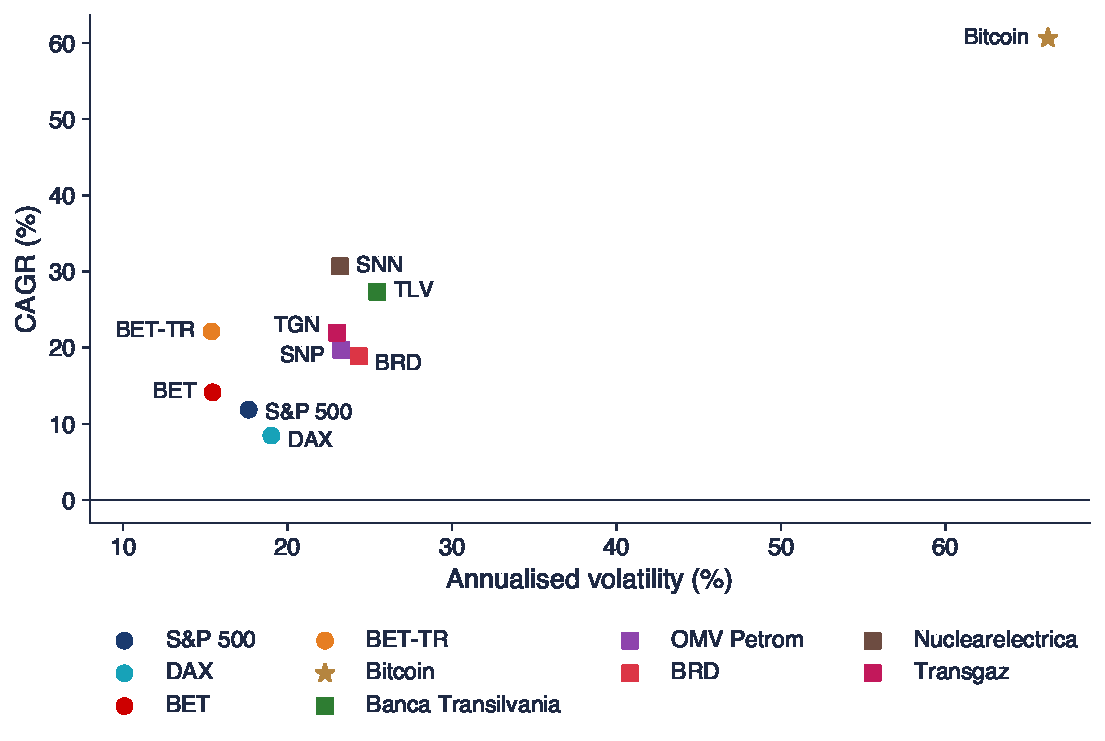
\includegraphics[width=\linewidth,height=0.80\textheight,keepaspectratio]{sfm_ch1_risk_return.pdf}
\end{center}
\end{column}
\begin{column}{0.40\textwidth}
\begin{itemize}
    \item Horizontal: annualised volatility; vertical: CAGR
    \item Best by CAGR: Bitcoin; by Sharpe: BET-TR; by Sortino: SNN; by Calmar: SNN
    \item Lowest volatility: BET-TR; shallowest MDD: BET-TR
    \item The ranking depends on the indicator: always say which one you use
\end{itemize}
\end{column}
\end{columns}
\quantlet{SFM\_ch1\_performance}{\qlurl{SFM_ch1_performance}}
\end{frame}

\begin{frame}{Recap: Performance Indicators}
\itemsize{\small}
\begin{itemize}
    \item CAGR (growth), volatility (risk), Sharpe and Sortino (return per unit of risk)
    \item MDD and Calmar: the worst fall, which the investor actually lives through
    \item Volatility drag: $\mu_{\text{log}} \approx \mu_{\text{arith}} - \sigma^2/2$, growth is below the arithmetic mean
    \item Every indicator is an estimate: compare differences with their standard errors
\end{itemize}
\end{frame}


%=============================================================================
\section{AI for Scientific Discovery}
%=============================================================================

\begin{frame}{An Open Question}
\itemsize{\small}
\begin{itemize}
    \item \textbf{Do Sharpe ratios persist?}
    \begin{itemize}
        \item if a BVB stock had a high Sharpe ratio in 2015--2020, did it also have one in 2021--2026?
        \item if not, ranking funds or stocks by past Sharpe ratios is of little use to an investor
    \end{itemize}
    \item Why it is open: short samples, few stocks, and a standard error of about $0.4$ for a Sharpe ratio estimated on half of our sample
    \item Related evidence: many published return patterns do not survive new data \refHLZ
    \item AI tools can speed up such a study; they do not replace checking it \refWang
\end{itemize}
\end{frame}

\begin{frame}{How AI Could Help}
\itemsize{\small}
\begin{itemize}
    \item \textbf{Literature}: list papers on the persistence of performance and summarise their methods
    \item \textbf{Code}: draft a Python function for rolling Sharpe ratios on the course data
    \item \textbf{Robustness}: propose other windows, other indicators (Sortino, Calmar), other markets
    \item \textbf{Explanation}: turn a table of results into a first draft of the interpretation
    \item Example prompt
    \begin{itemize}
        \item \aiprompt{Write a Python function that computes the annualised Sharpe ratio of daily simple returns on non-overlapping 3-year windows, with the Lo (2002) standard error.}
    \end{itemize}
\end{itemize}
\end{frame}

\begin{frame}{What to Check}
\itemsize{\small}
\begin{itemize}
    \item Data: adjusted close for stocks, the same calendar for all assets, the right period
    \item Formulas: the annualisation factor ($\sqrt{252}$ vs $\sqrt{365}$), simple vs log returns, $n$ vs $n - 1$
    \item Numbers: recompute two or three values on small examples or with a second method
    \item References: every cited paper must exist; check the DOI
    \item Selection: if you tried ten windows, say so; a backtest tried many times overfits \refBBLZ
\end{itemize}
\end{frame}

\begin{frame}{Project Seed}
\itemsize{\small}
\begin{itemize}
    \item \textbf{Question}: do Sharpe ratios of BVB stocks persist from one period to the next?
    \begin{itemize}
        \item data: adjusted closes of 10--15 BVB stocks, 2010--2026, from the course data
    \end{itemize}
    \item Steps
    \begin{itemize}
        \item split the sample into two halves; compute Sharpe ratios and their standard errors in each
        \item measure persistence with the rank correlation between the two halves
        \item repeat with Sortino and Calmar ratios
    \end{itemize}
    \item Deliverable: one table, one chart, and a paragraph on what the data can and cannot show
    \item Declare any AI use, and list the errors of the AI that you corrected
\end{itemize}
\end{frame}


%=============================================================================
\section{Summary}
%=============================================================================

\begin{frame}{Key Takeaways}
\itemsize{\small}
\begin{itemize}
    \item Check the data first: source, adjusted prices, calendar, jumps
    \item Log returns add over time; simple returns add across assets
    \item Annualise with the actual frequency: mean $\times\,q$, volatility $\times\sqrt{q}$
    \item Returns have heavy tails, negative skewness and changing volatility
    \item Judge performance with several indicators: CAGR, volatility, Sharpe, Sortino, MDD, Calmar
    \item Volatility costs growth: $\sigma^2/2$ a year
    \item Mean returns and Sharpe ratios are imprecise: report standard errors
\end{itemize}
\end{frame}

\begin{frame}{Key Formulas}
\itemsize{\small}
\begin{center}
\footnotesize
\begin{tabular}{ll}
\toprule
\textbf{Quantity} & \textbf{Formula} \\
\midrule
Simple return & $R_t = P_t/P_{t-1} - 1$ \\
Log return & $r_t = \ln(P_t/P_{t-1}) = \ln(1 + R_t)$ \\
$k$-period returns & $1 + R_t(k) = \prod_{j=0}^{k-1}(1 + R_{t-j})$, \quad $r_t(k) = \sum_{j=0}^{k-1} r_{t-j}$ \\
Portfolio & $R_p = \sum_i w_i R_i$ \\
Annualisation & $\mu_{\text{year}} = q\,\mu$, \quad $\sigma_{\text{year}} = \sqrt{q}\,\sigma$ \\
CAGR & $(P_T/P_0)^{1/Y} - 1$ \\
Sharpe, Sortino & $(\mu - r_f)/\sigma$, \quad $(\mu - \tau)/\sigma_D$ \\
MDD, Calmar & $\min_t \big(P_t / \max_{s \le t} P_s - 1\big)$, \quad $\text{CAGR}/|\text{MDD}|$ \\
Volatility drag & $\mu_{\text{log}} \approx \mu_{\text{arith}} - \sigma^2/2$ \\
SE of mean, of Sharpe & $\sigma_{\text{year}}/\sqrt{Y}$, \quad $\sqrt{(1 + \text{SR}^2/2)/n}$ \\
\bottomrule
\end{tabular}
\end{center}
\end{frame}

\begin{frame}{Check Yourself}
\itemsize{\small}
\begin{itemize}
    \item \textbf{Question}: a fund reports daily log returns with mean 0.05\% and standard deviation 1\%; what are its annual mean and volatility?
    \begin{itemize}
        \item \textbf{Answer}: $252 \times 0.05\% = 12.6\%$ and $\sqrt{252} \times 1\% = 15.9\%$
    \end{itemize}
    \item \textbf{Question}: why is the arithmetic mean return of Bitcoin far above its CAGR?
    \begin{itemize}
        \item \textbf{Answer}: the volatility drag $\sigma^2/2$ is large when $\sigma$ is large
    \end{itemize}
    \item \textbf{Question}: an index falls by 60\%; what gain does it need to recover?
    \begin{itemize}
        \item \textbf{Answer}: $0.6/0.4 = 150\%$
    \end{itemize}
    \item Next: \sfmchlink{https://danpele.github.io/SFM/EN/Courses/chapter2_classical_distributions_stylised_facts.pdf}{Chapter 2}, classical distributions and stylised facts of returns
\end{itemize}
\end{frame}


%=============================================================================
\section{References}
%=============================================================================

\begin{frame}{References (1/2)}
\itemsize{\tiny}
\begin{itemize}
    \item Bailey, D.H., Borwein, J.M., López de Prado, M., Zhu, Q.J. (2014). \href{https://doi.org/10.1090/noti1105}{Pseudo-mathematics and financial charlatanism: the effects of backtest overfitting on out-of-sample performance}. \textit{Notices of the American Mathematical Society}, 61(5), 458--471.
    \item Bailey, D.H., López de Prado, M. (2014). \href{https://doi.org/10.3905/jpm.2014.40.5.094}{The deflated Sharpe ratio: correcting for selection bias, backtest overfitting, and non-normality}. \textit{Journal of Portfolio Management}, 40(5), 94--107.
    \item Booth, D.G., Fama, E.F. (1992). \href{https://doi.org/10.2469/faj.v48.n3.26}{Diversification returns and asset contributions}. \textit{Financial Analysts Journal}, 48(3), 26--32.
    \item Borak, S., Härdle, W.K., López-Cabrera, B. (2013). \href{https://doi.org/10.1007/978-3-642-33929-5}{\textit{Statistics of Financial Markets: Exercises and Solutions}}, 2nd ed. Springer.
    \item Brown, S.J., Goetzmann, W., Ibbotson, R.G., Ross, S.A. (1992). \href{https://doi.org/10.1093/rfs/5.4.553}{Survivorship bias in performance studies}. \textit{Review of Financial Studies}, 5(4), 553--580.
    \item Campbell, J.Y., Lo, A.W., MacKinlay, A.C. (1997). \href{https://doi.org/10.1515/9781400830213}{\textit{The Econometrics of Financial Markets}}. Princeton University Press.
    \item Cont, R. (2001). \href{https://doi.org/10.1080/713665670}{Empirical properties of asset returns: stylized facts and statistical issues}. \textit{Quantitative Finance}, 1(2), 223--236.
    \item Dickey, D.A., Fuller, W.A. (1979). \href{https://doi.org/10.1080/01621459.1979.10482531}{Distribution of the estimators for autoregressive time series with a unit root}. \textit{Journal of the American Statistical Association}, 74(366), 427--431.
    \item Franke, J., Härdle, W.K., Hafner, C.M. (2019). \href{https://doi.org/10.1007/978-3-030-13751-9}{\textit{Statistics of Financial Markets: An Introduction}}, 5th ed. Springer.
    \item Harvey, C.R., Liu, Y., Zhu, H. (2016). \href{https://doi.org/10.1093/rfs/hhv059}{\ldots and the cross-section of expected returns}. \textit{Review of Financial Studies}, 29(1), 5--68.
    \item Lo, A.W. (2002). \href{https://doi.org/10.2469/faj.v58.n4.2453}{The statistics of Sharpe ratios}. \textit{Financial Analysts Journal}, 58(4), 36--52.
    \item Magdon-Ismail, M., Atiya, A.F., Pratap, A., Abu-Mostafa, Y.S. (2004). \href{https://doi.org/10.1239/jap/1077134674}{On the maximum drawdown of a Brownian motion}. \textit{Journal of Applied Probability}, 41(1), 147--161.
    \item Pele, D.T., Mazurencu-Marinescu, M. (2012). \href{https://doi.org/10.1016/j.sbspro.2012.09.1030}{Modelling stock market crashes: the case of Bucharest Stock Exchange}. \textit{Procedia -- Social and Behavioral Sciences}, 58, 533--542.
    \item Sharpe, W.F. (1966). \href{https://doi.org/10.1086/294846}{Mutual fund performance}. \textit{Journal of Business}, 39(S1), 119--138.
    \item Sharpe, W.F. (1994). \href{https://doi.org/10.3905/jpm.1994.409501}{The Sharpe ratio}. \textit{Journal of Portfolio Management}, 21(1), 49--58.
    \item Sortino, F.A., van der Meer, R. (1991). \href{https://doi.org/10.3905/jpm.1991.409343}{Downside risk}. \textit{Journal of Portfolio Management}, 17(4), 27--31.
\end{itemize}
\end{frame}

\begin{frame}{References (2/2)}
\itemsize{\tiny}
\begin{itemize}
    \item Tsay, R.S. (2010). \href{https://doi.org/10.1002/9780470644560}{\textit{Analysis of Financial Time Series}}, 3rd ed. Wiley.
    \item Wang, H., Fu, T., Du, Y., Gao, W., et al. (2023). \href{https://doi.org/10.1038/s41586-023-06221-2}{Scientific discovery in the age of artificial intelligence}. \textit{Nature}, 620, 47--60.
\end{itemize}
\end{frame}

\end{document}
